% Options for packages loaded elsewhere
\PassOptionsToPackage{unicode}{hyperref}
\PassOptionsToPackage{hyphens}{url}
\PassOptionsToPackage{dvipsnames,svgnames,x11names}{xcolor}
%
\documentclass[
]{article}

\usepackage{amsmath,amssymb}
\usepackage{iftex}
\ifPDFTeX
  \usepackage[T1]{fontenc}
  \usepackage[utf8]{inputenc}
  \usepackage{textcomp} % provide euro and other symbols
\else % if luatex or xetex
  \usepackage{unicode-math}
  \defaultfontfeatures{Scale=MatchLowercase}
  \defaultfontfeatures[\rmfamily]{Ligatures=TeX,Scale=1}
\fi
\usepackage{lmodern}
\ifPDFTeX\else  
    % xetex/luatex font selection
\fi
% Use upquote if available, for straight quotes in verbatim environments
\IfFileExists{upquote.sty}{\usepackage{upquote}}{}
\IfFileExists{microtype.sty}{% use microtype if available
  \usepackage[]{microtype}
  \UseMicrotypeSet[protrusion]{basicmath} % disable protrusion for tt fonts
}{}
\makeatletter
\@ifundefined{KOMAClassName}{% if non-KOMA class
  \IfFileExists{parskip.sty}{%
    \usepackage{parskip}
  }{% else
    \setlength{\parindent}{0pt}
    \setlength{\parskip}{6pt plus 2pt minus 1pt}}
}{% if KOMA class
  \KOMAoptions{parskip=half}}
\makeatother
\usepackage{xcolor}
\setlength{\emergencystretch}{3em} % prevent overfull lines
\setcounter{secnumdepth}{-\maxdimen} % remove section numbering
% Make \paragraph and \subparagraph free-standing
\ifx\paragraph\undefined\else
  \let\oldparagraph\paragraph
  \renewcommand{\paragraph}[1]{\oldparagraph{#1}\mbox{}}
\fi
\ifx\subparagraph\undefined\else
  \let\oldsubparagraph\subparagraph
  \renewcommand{\subparagraph}[1]{\oldsubparagraph{#1}\mbox{}}
\fi


\providecommand{\tightlist}{%
  \setlength{\itemsep}{0pt}\setlength{\parskip}{0pt}}\usepackage{longtable,booktabs,array}
\usepackage{calc} % for calculating minipage widths
% Correct order of tables after \paragraph or \subparagraph
\usepackage{etoolbox}
\makeatletter
\patchcmd\longtable{\par}{\if@noskipsec\mbox{}\fi\par}{}{}
\makeatother
% Allow footnotes in longtable head/foot
\IfFileExists{footnotehyper.sty}{\usepackage{footnotehyper}}{\usepackage{footnote}}
\makesavenoteenv{longtable}
\usepackage{graphicx}
\makeatletter
\def\maxwidth{\ifdim\Gin@nat@width>\linewidth\linewidth\else\Gin@nat@width\fi}
\def\maxheight{\ifdim\Gin@nat@height>\textheight\textheight\else\Gin@nat@height\fi}
\makeatother
% Scale images if necessary, so that they will not overflow the page
% margins by default, and it is still possible to overwrite the defaults
% using explicit options in \includegraphics[width, height, ...]{}
\setkeys{Gin}{width=\maxwidth,height=\maxheight,keepaspectratio}
% Set default figure placement to htbp
\makeatletter
\def\fps@figure{htbp}
\makeatother

\usepackage{booktabs}
\usepackage{longtable}
\usepackage{array}
\usepackage{multirow}
\usepackage{wrapfig}
\usepackage{float}
\usepackage{colortbl}
\usepackage{pdflscape}
\usepackage{tabu}
\usepackage{threeparttable}
\usepackage{threeparttablex}
\usepackage[normalem]{ulem}
\usepackage{makecell}
\usepackage{xcolor}
\usepackage{fancyhdr}
\pagestyle{fancy}
\fancyhf{}
\fancyfoot[C]{\thepage}
\makeatletter
\makeatother
\makeatletter
\makeatother
\makeatletter
\@ifpackageloaded{caption}{}{\usepackage{caption}}
\AtBeginDocument{%
\ifdefined\contentsname
  \renewcommand*\contentsname{Table of contents}
\else
  \newcommand\contentsname{Table of contents}
\fi
\ifdefined\listfigurename
  \renewcommand*\listfigurename{List of Figures}
\else
  \newcommand\listfigurename{List of Figures}
\fi
\ifdefined\listtablename
  \renewcommand*\listtablename{List of Tables}
\else
  \newcommand\listtablename{List of Tables}
\fi
\ifdefined\figurename
  \renewcommand*\figurename{Figure}
\else
  \newcommand\figurename{Figure}
\fi
\ifdefined\tablename
  \renewcommand*\tablename{Table}
\else
  \newcommand\tablename{Table}
\fi
}
\@ifpackageloaded{float}{}{\usepackage{float}}
\floatstyle{ruled}
\@ifundefined{c@chapter}{\newfloat{codelisting}{h}{lop}}{\newfloat{codelisting}{h}{lop}[chapter]}
\floatname{codelisting}{Listing}
\newcommand*\listoflistings{\listof{codelisting}{List of Listings}}
\makeatother
\makeatletter
\@ifpackageloaded{caption}{}{\usepackage{caption}}
\@ifpackageloaded{subcaption}{}{\usepackage{subcaption}}
\makeatother
\makeatletter
\@ifpackageloaded{tcolorbox}{}{\usepackage[skins,breakable]{tcolorbox}}
\makeatother
\makeatletter
\@ifundefined{shadecolor}{\definecolor{shadecolor}{rgb}{.97, .97, .97}}
\makeatother
\makeatletter
\makeatother
\makeatletter
\makeatother
\ifLuaTeX
  \usepackage{selnolig}  % disable illegal ligatures
\fi
\IfFileExists{bookmark.sty}{\usepackage{bookmark}}{\usepackage{hyperref}}
\IfFileExists{xurl.sty}{\usepackage{xurl}}{} % add URL line breaks if available
\urlstyle{same} % disable monospaced font for URLs
\hypersetup{
  pdftitle={Benthic Invertebrates Report},
  colorlinks=true,
  linkcolor={blue},
  filecolor={Maroon},
  citecolor={Blue},
  urlcolor={Blue},
  pdfcreator={LaTeX via pandoc}}

\title{Benthic Invertebrates Report}
\author{}
\date{}

\begin{document}
\maketitle
\ifdefined\Shaded\renewenvironment{Shaded}{\begin{tcolorbox}[interior hidden, enhanced, sharp corners, frame hidden, breakable, boxrule=0pt, borderline west={3pt}{0pt}{shadecolor}]}{\end{tcolorbox}}\fi

\renewcommand*\contentsname{Contents}
{
\hypersetup{linkcolor=}
\setcounter{tocdepth}{3}
\tableofcontents
}
\hypertarget{introduction}{%
\subsection{Introduction}\label{introduction}}

Benthic monitoring conducted by the California Department of Water
Resources (DWR) since 1975 has documented changes in the composition,
density, and distribution of the macrobenthic biota inhabiting the upper
San Francisco Estuary. This monitoring is performed by the Environmental
Monitoring Program (EMP) as part of the Interagency Ecological Program
(IEP) and is one component of the biological monitoring mandated by
Water Right Decision D-1641. Since benthic species respond to changes in
physical factors such as freshwater inflows, salinity, and substrate
composition, benthic community data provides an indication of physical
changes occurring within the Estuary. Benthic monitoring is an important
component of the EMP because operation of the State Water Project can
change the Estuary's flow characteristics, affecting the density and
distribution of benthic biota. Benthic monitoring data is also used to
detect and document the presence of new, non-native species in the Upper
Estuary, such as the 1986 arrival and subsequent wide spread of the
overbite clam, Potamocorbula amurensis. This report describes the
results of these monitoring efforts for water year 2023 (October 1st
2022 through September 30th 2023) which was classified as a wet year in
the Sacramento and San Joaquin Valleys
\href{https://cdec.water.ca.gov/reportapp/javareports?name=WSIHIST}{(source)}.

\hypertarget{methods}{%
\subsection{Methods}\label{methods}}

Benthic monitoring was conducted monthly at 10 sampling sites
distributed throughout the Estuary, from San Pablo Bay upstream through
the Sacramento-San Joaquin Delta (Figure~\ref{fig-stations};
Table~\ref{tbl-stations}). EMP staff collected four bottom grab samples
at each station using a Ponar dredge with a sampling area of 0.052
\(m^2\). The four replicate grab samples were analyzed for benthic
macrofauna by Hydrozoology, a private laboratory under contract with
DWR. All organisms were identified to the lowest taxon possible and
enumerated.

\begin{figure}

{\centering \includegraphics[width=0.9\textwidth,height=\textheight]{../figures/benthic_station_map.png}

}

\caption{\label{fig-stations}Map of EMP's benthic field sites.}

\end{figure}

\begin{table}

\caption{\label{tbl-stations}\textbf{?(caption)}}\begin{minipage}[t]{\linewidth}
\subcaption{\label{tbl-stations-1}}

{\centering 

\begingroup\fontsize{14}{16}\selectfont

}

\end{minipage}%
\newline
\begin{minipage}[t]{\linewidth}
\subcaption{\label{tbl-stations-2}}

{\centering 

\begin{longtabu} to \linewidth {>{\centering\arraybackslash}p{33.3333333333333%}>{\centering\arraybackslash}p{33.3333333333333%}>{\centering\arraybackslash}p{33.3333333333333%}}
\toprule
Region & WY Index & Stations\\
\midrule
Carquinez & Sacramento & NZ002, NZ004\\
Central Delta & San Joaquin & D16, D19, D26, D28A\\
Confluence & Sacramento & D4, D10, D12, D22\\
North Delta & Sacramento & C3A, NZ068\\
San Pablo Bay & Sacramento & D41, D41A, NZ325\\
\addlinespace
South Delta & San Joaquin & C9, C10A, MD10A, P8\\
Suisun \& Grizzly Bays & Sacramento & D6, D7, D8\\
Suisun Marsh & Sacramento & NZ032, NZS42\\
\bottomrule
\end{longtabu}
\endgroup{}

}

\end{minipage}%

\end{table}

The 10 most common genera were determined by summing the normalized
organism counts across all stations and months for each genus. For the
bar graphs, the data is reported as the average~ organism catch per unit
effort (CPUE).~ This was calculated as the organism count per replicate
grab, converted to organisms per m\textsuperscript{2} (each grab is
0.052m\textsuperscript{2}), averaged across replicates for each station
in each month and aggregated by phylum.

For more in-depth methodology, see
\href{https://portal.edirepository.org/nis/metadataviewer?packageid=edi.1320.6}{here}.

\hypertarget{overall-results}{%
\subsection{Overall Results}\label{overall-results}}

The benthic fauna collected in FY2023 comprised nine phyla: Annelida
(37\% of total organisms), Arthropoda (31\%) and Mollusca (31\%), with
Phoronida, Nematoda, Chordata, Platyhelminthes, Cnidaria, and Nemertea
each representing 1\% or less of total organisms. Of the 185 benthic
species collected in WY 2023, the ten most abundant species represented
80\% of all individuals collected throughout the year
(Figure~\ref{fig-abund}). These include three species of amphipod, two
clams, three oligochate worms, one polychate worm, and one cumacean
arthropod (also known as a comma shrimp, although it is not actually a
shrimp). Only three species in this group (the
amphipods~\emph{Americorophium spinicorne} and \emph{Hyalella sp.}, and
the oligochaete worm \emph{Ilyodrilus franzti}) are native to this
estuary. The rest of the top ten species are non-native or are
cosmopolitan species of unknown origin. Refer to Fields and Messer
(1999) for descriptions of the habitat requirements, physical
attributes, and feeding methods of many of these species.

In the site descriptions that follow, most species densities are
reported as the annual densities of individuals/m\textsuperscript{2},
sometimes noting dramatic seasonal peaks. Some species, especially
arthropods, display strong seasonal variability with peak monthly
densities several times higher than their annual densities. In these
cases, we reported the time and magnitude of the peaks as well as the
annual densities. Please note that the station P8 was not sampled in
December 2022 due to heavy fog, and comparisons to other years' average
annual densities or seasonal patterns should take this omission into
account.

\begin{figure}

{\centering 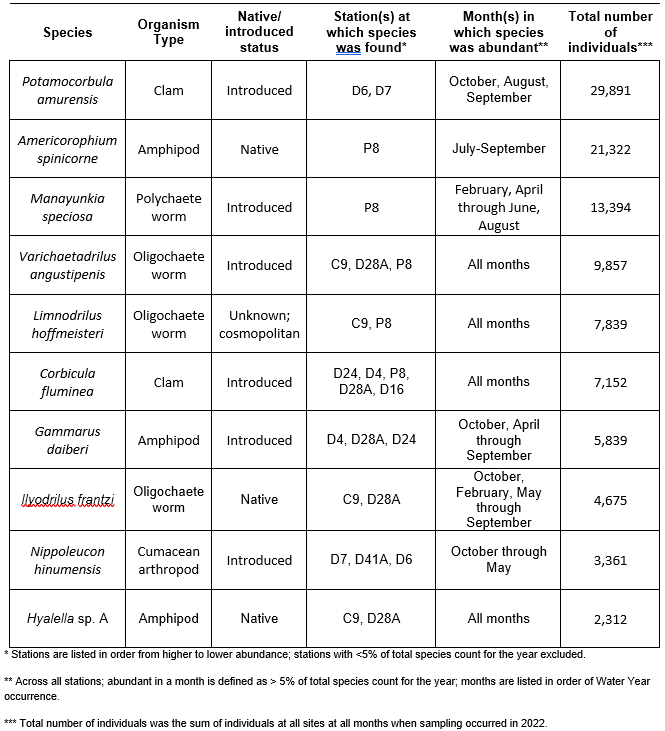
\includegraphics[width=0.9\textwidth,height=\textheight]{../figures/species_list.png}

}

\caption{\label{fig-abund}List of ten most numerous benthic invertebrate
species found at EMP sites.}

\end{figure}

\hypertarget{regional-results}{%
\subsection{Regional Results}\label{regional-results}}

\hypertarget{central-delta-d16-d28a}{%
\subsubsection{Central Delta (D16, D28A)}\label{central-delta-d16-d28a}}

The benthic monitoring program sampled at two stations, in the Central
Delta, D16 and D28. Site D16 is on the lower San Joaquin River near
Twitchell Island (Figure~\ref{fig-stations}). There were 15 species in
four phyla at D16 in WY 2023, split between Mollusca (62\% of all
organisms collected in 2023) and Arthropoda (37\%)
(Figure~\ref{fig-benthic_d16}). The most abundant species at D16 was the
clam~\emph{Corbicula fluminea}~which accounted for 58\% of all organisms
in 2022, with an average annual density of 146
individuals/m\textsuperscript{2}~and peaks in May and August 2023. The
amphipod~\emph{Gammarus daiberi}~was the second most abundant organism,
accounting for 25\% of all individuals, with an average annual density
of 62 individuals/m\textsuperscript{2}~and a peak in October 2022 of 230
individuals/m\textsuperscript{2} and another in February of 169
individuals/m\textsuperscript{2}.~ Much of the rest of the community was
a combination of various species of amphipods and snails at lower
densities. The total number of organisms at D16 in WY 2023 continued the
trend of very low numbers compared with other years in the previous
decade. In particular, WY 2020-2023 saw very low numbers of the
amphipod~\emph{Americorophium spinicorne}, which was seen in very high
numbers at D16 from 2015-2018.

The site on Old River near Rancho Del Rio is known as D28A
(Figure~\ref{fig-stations}). In WY 2023, there were 58 species in seven
phyla at D28A. The most abundant phylum was Annelida, followed by
Arthropoda and Mollusca (55\%, 33\%, and 12\% of all organisms,
respectively) (Figure~\ref{fig-benthic_d28a}). The most abundant species
was the oligochaete worm~\emph{Variachaetadrilus angustipenis} with an
average density of 1,494 individuals/m\textsuperscript{2} and high
densities between December 2022 and May 2023, followed by the ostracod
crustacean \emph{Cyprideis} sp. A with an average density of 767
individuals/m\textsuperscript{2} and higher densities between December
2022 and March 2023.~ The Asian clam \emph{Corbicula fluminea} had an
annual average density of 356 individuals/m\textsuperscript{2} that grew
from April through July, likely via seasonal recruitment.~ While D28A
had similarly high species richness in WY 2023 to other years, a few
notable differences were fewer of the amphipods \emph{Gammarus daiberi}
and \emph{Americorophium spinicorne}, which were both more numerous in
2013, 2014, and 2022 than now, as well as many fewer of the sabellid
worm \emph{Manayunkia speciosa}, which was the most numerous organism at
D28A in several years of the past decade but in WY 2023 comprised just
3.5\% of all organisms found here.

\begin{figure}

{\centering 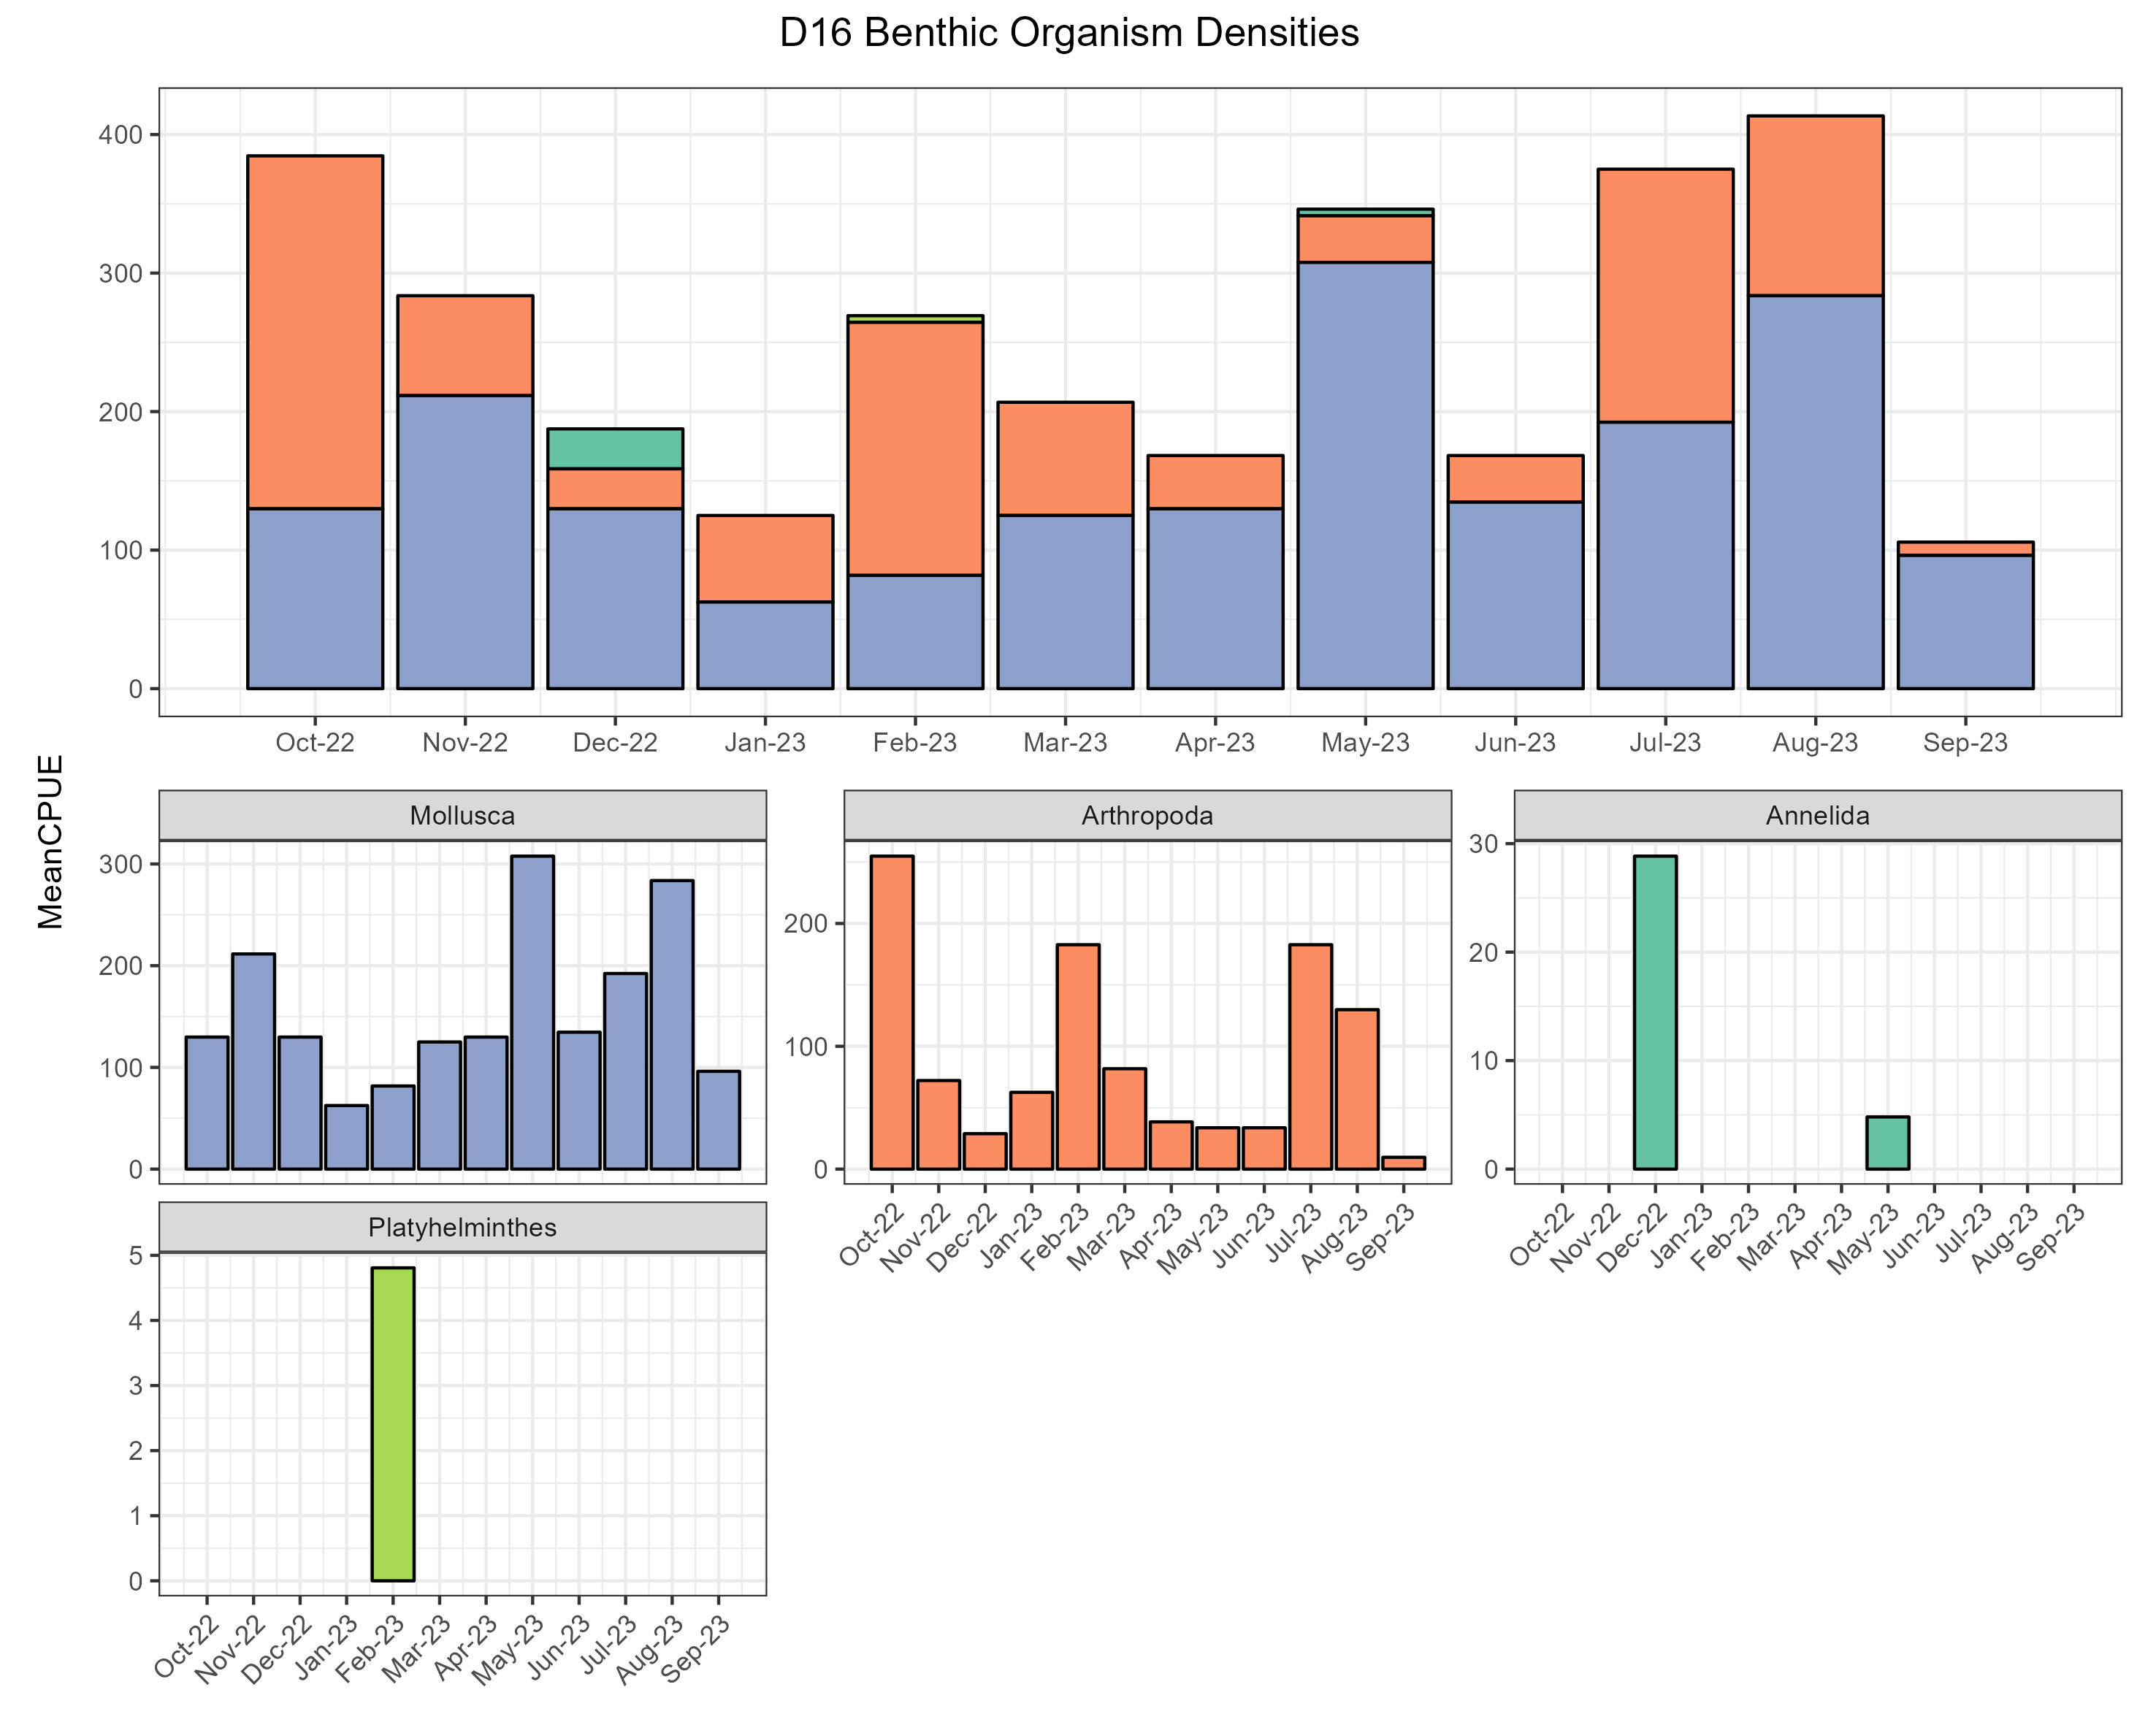
\includegraphics[width=9.84in,height=\textheight]{../figures/benthic_bar_d16.jpg}

}

\caption{\label{fig-benthic_d16}Density of benthic organisms, by month,
collected at station D16.}

\end{figure}

\begin{figure}

{\centering 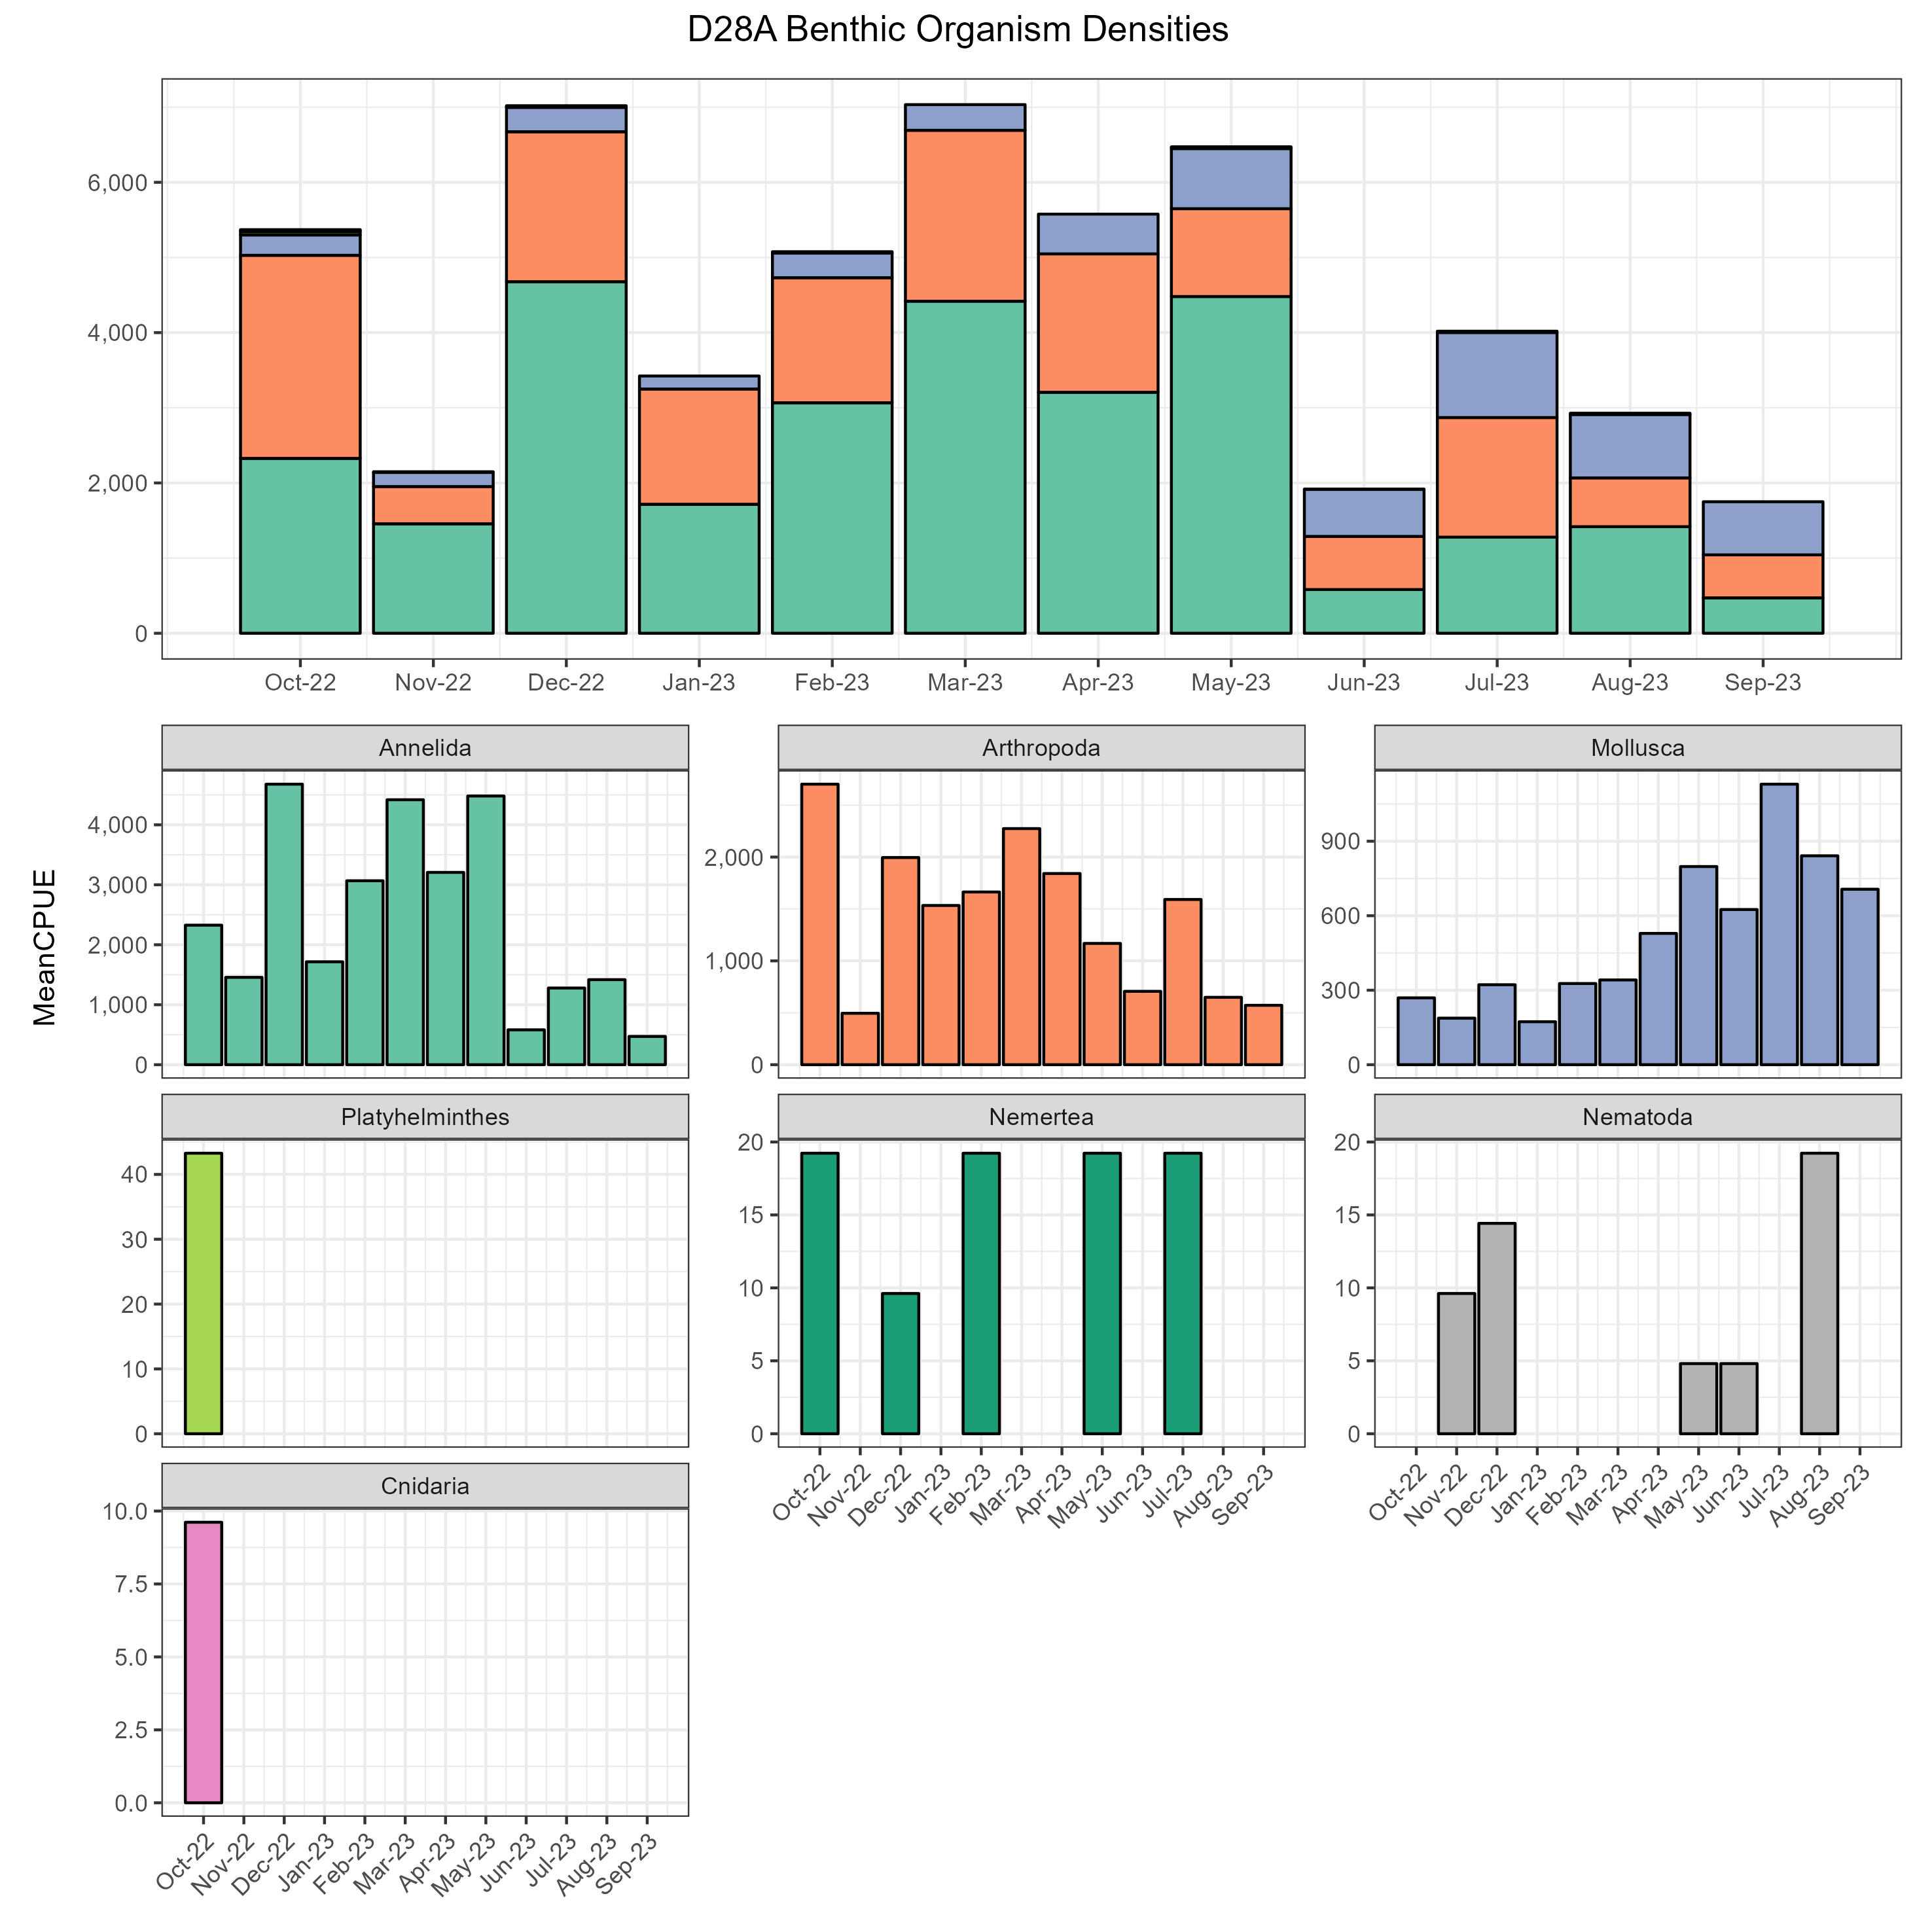
\includegraphics[width=9.84in,height=\textheight]{../figures/benthic_bar_d28a.jpg}

}

\caption{\label{fig-benthic_d28a}Density of benthic organisms, by month,
collected at station D28A.}

\end{figure}

\hypertarget{confluence-d4}{%
\subsubsection{Confluence (D4)}\label{confluence-d4}}

Site D4 is located near the confluence of the Sacramento and San Joaquin
Rivers, just north of Point Sacramento (Figure~\ref{fig-stations}).
There were 41 species in six phyla at D4, and in WY 2023 this was the
site with the highest number of organisms. Arthropoda was by far the
most abundant phylum (88\% of all organisms) followed by Annelida (7\%
of all organisms) and Mollusca (6\% of all organisms)
(Figure~\ref{fig-benthic_d4}). The native amphipod~\emph{Americorophium
spinicorne}~was the most abundant species at this station and made up
slightly over 71\% of all individual organisms in WY 2023 with a
dramatic seasonal peak of 55,279 individuals/m\textsuperscript{2}~in
August 2023 and an annual average of 8,436
individuals/m\textsuperscript{2}, the highest annual average in a
decade. The non-native amphipod \emph{Gammarus daiberi} had an annual
average of 1,562 individuals/m\textsuperscript{2}, which was at low
density before increasing~ in June to a seasonal peak in September of
5,380 individuals/m\textsuperscript{2}.~ The invasive clam
\emph{Corbicula fluminea} also saw a summer seasonal increase, with a
high in August of 1,788 and an annual average of
471~individuals/m\textsuperscript{2}.

Because of D4's position at the front of saltwater and freshwater mixing
in the estuary, we often see a shift from the freshwater
clam~\emph{Corbicula fluminea}~to more
brackish-water~\emph{Potamocorbula amurensis}~following dry years, and
the reverse following wet years.~ The drought of 2018-2022 led to high
\emph{Potamocorbula} numbers, which abruptly crashed down in WY 2023
while \emph{Corbicula} increased modestly. 2022 was also notable for its
rebound~of amphipod \emph{A. spinicorne}~in 2022 from the low of WY
2022.

\begin{figure}

{\centering 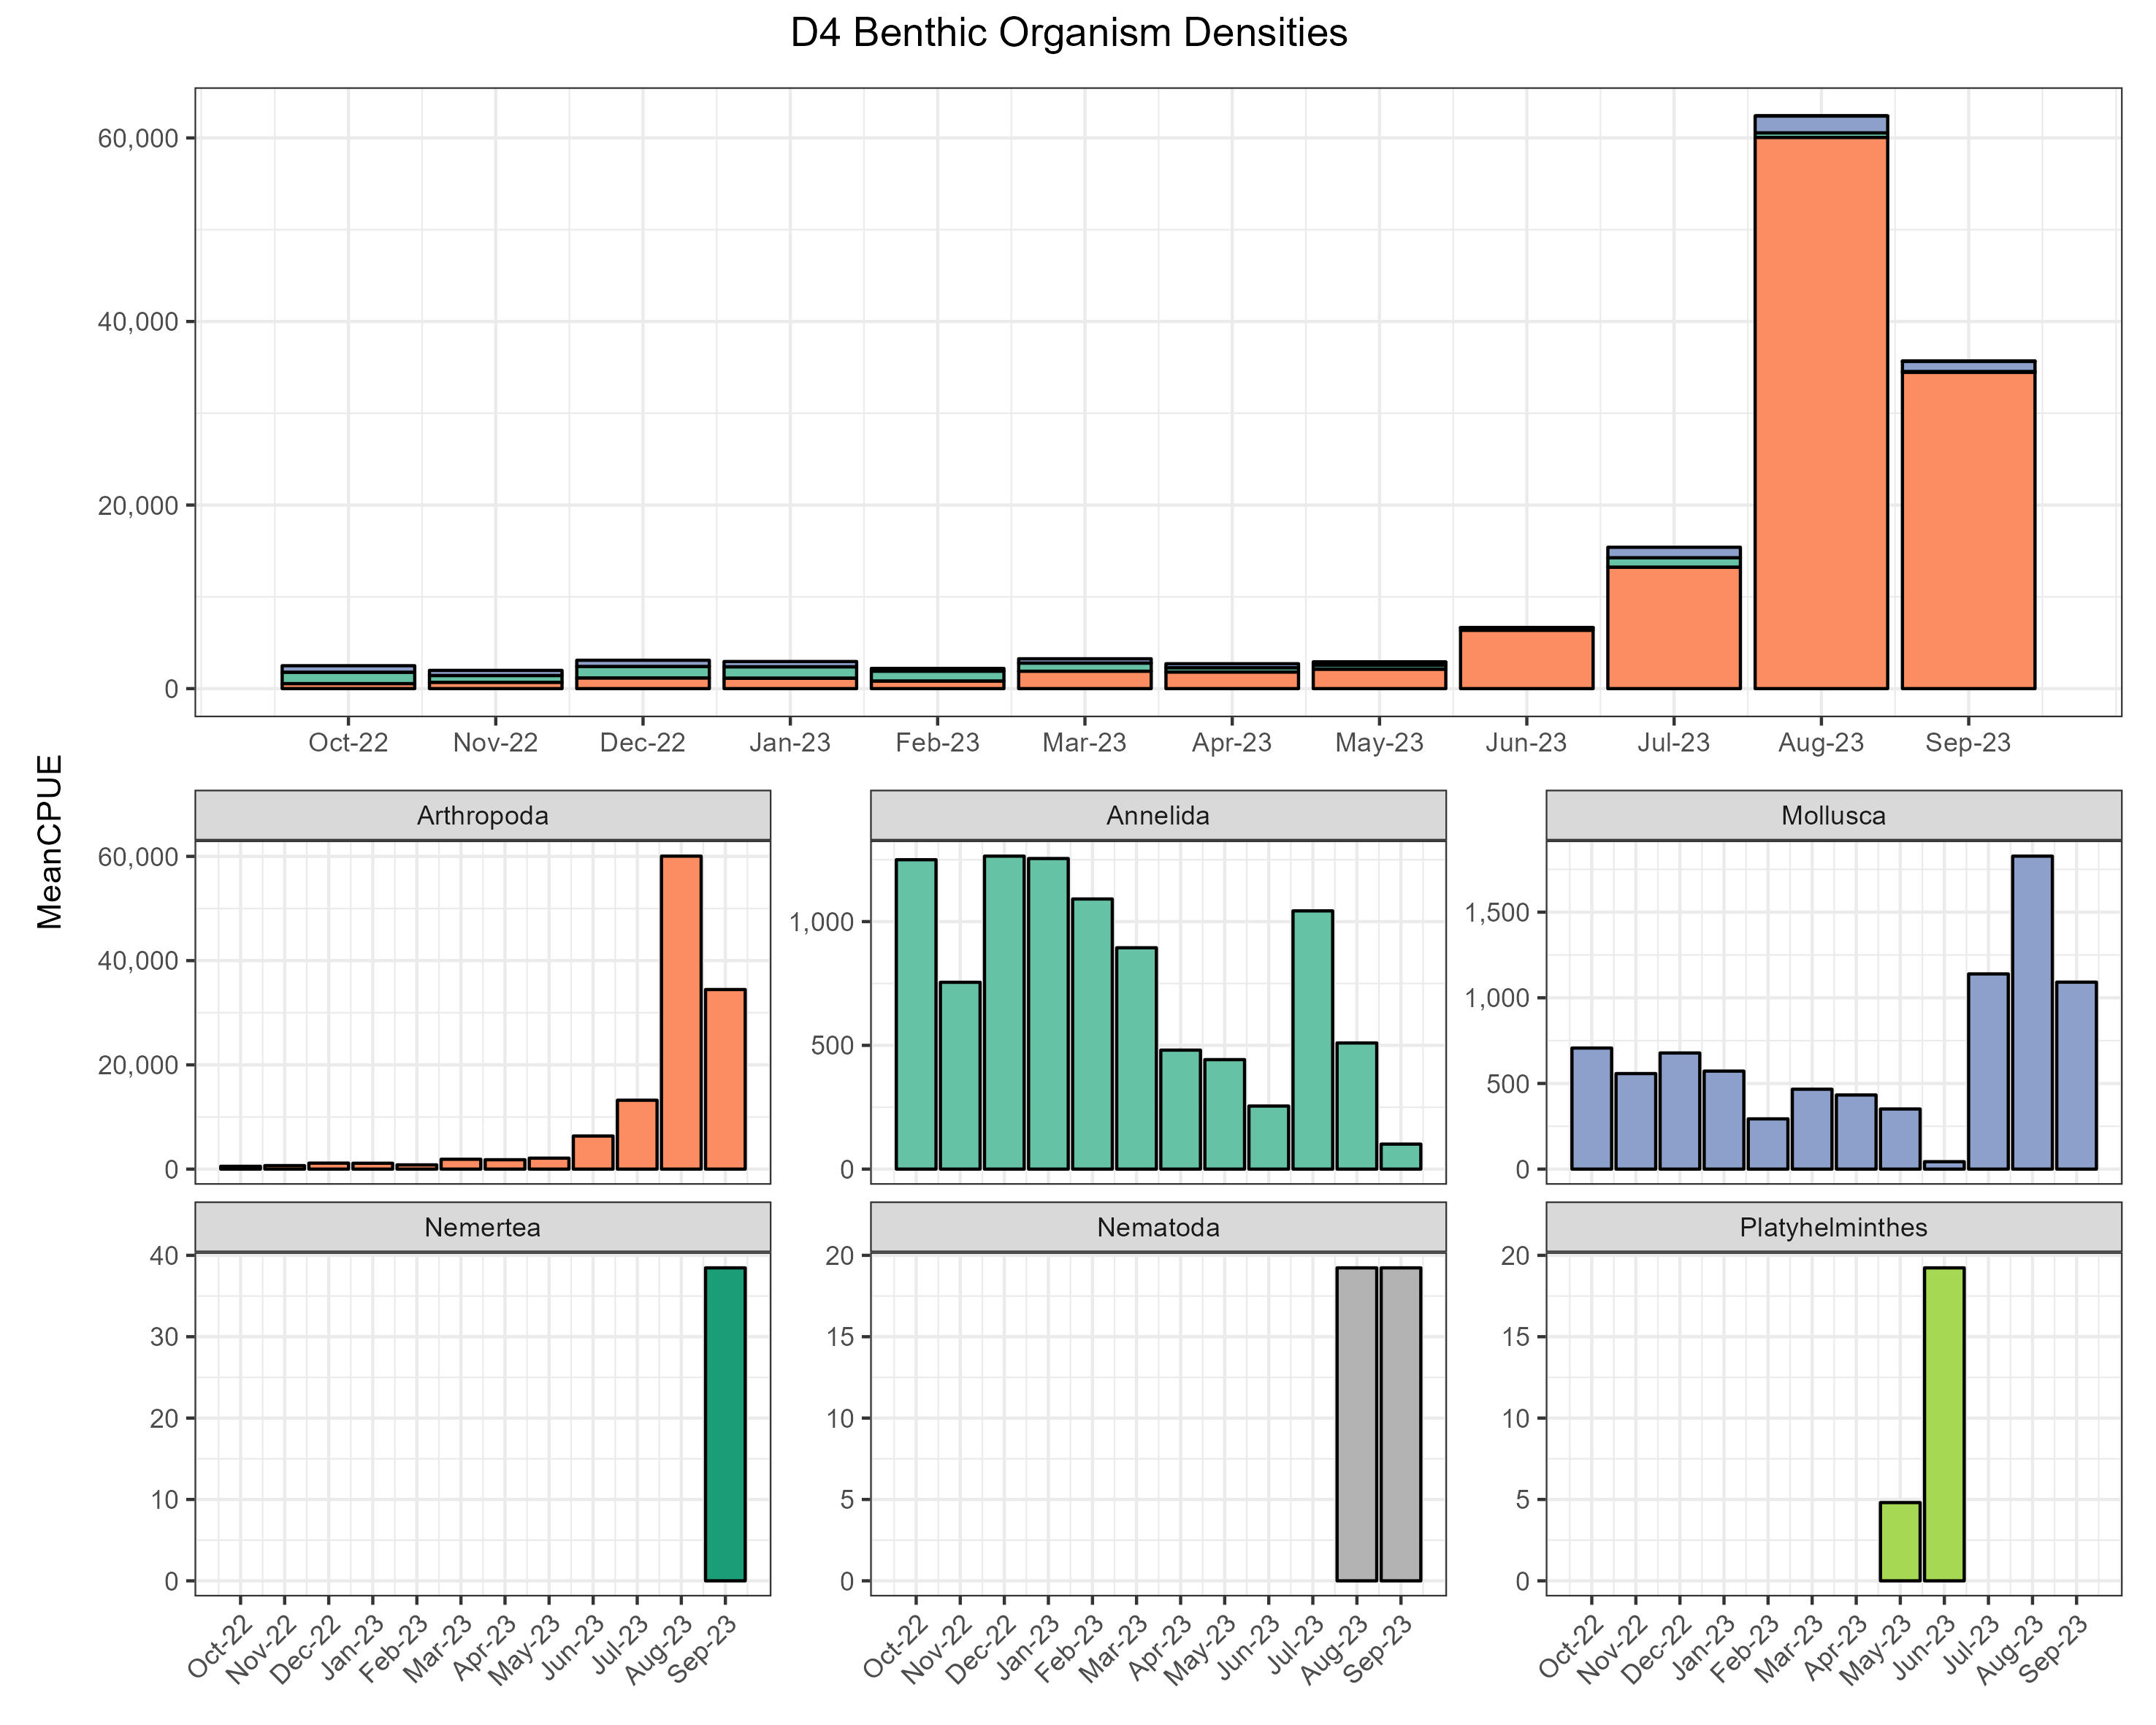
\includegraphics[width=9.84in,height=\textheight]{../figures/benthic_bar_d4.jpg}

}

\caption{\label{fig-benthic_d4}Density of benthic organisms, by month,
collected at station D4.}

\end{figure}

\hypertarget{san-pablo-bay-d41-d41a}{%
\subsubsection{San Pablo Bay (D41, D41A)}\label{san-pablo-bay-d41-d41a}}

The benthic monitoring program sampled at two stations in San Pablo Bay,
D41 and D41A. Station D41 is near Point Pinole
(Figure~\ref{fig-stations}) and has a benthic community primarily
comprised of marine organisms, especially in drier water years. There
were 76 species in seven phyla at D41 in WY 2023. Annelida was the most
abundant phylum (37\% of all organisms) followed by Phoronida (25\%),
Arthropoda (24\%) and Mollusca (10\%) (Figure~\ref{fig-benthic_d41}).
The single most abundant species was~the \emph{Phoronis harmeri}, a
native tube-dwelling filter-feeder from the small marine lophophorate
phylum Phoronida, with an average annual density of 490
individuals/m\textsuperscript{2} and representing 25\% of all organisms.
The second most abundant species was non-native amphipod~\emph{Ampelisa
abdita}, comprising 19\% of all organisms with 370
organisms/m\textsuperscript{2}, most of them in a very strong peak in
September 2023. The window shell clam~\emph{Theora lubrica,}~along with
the tube-dwelling polychate worm~\emph{Pseudopolydora kempi}~and the
polychaete worm~\emph{Scoletoma luti}, were the other species found in
notable densities. D41 overall community composition in 2021 was similar
to the preceding decade apart from the high numbers of Potamocorbula
amurensis from WY 2017-2019,~ and the decrease in the amphipod
\emph{Ampelisca abdita} from its very high levels in WY 2018-2021.~ This
pattern reinforces that higher-salinity water years such as 2021 see
increases in more marine species such as~\emph{Apelisca
abdita},~\emph{Phoronis harmeri}, and~\emph{Theora lubrica}~but lower
numbers of the clam~\emph{Potamocorbula amurensis}, which prefers more
brackish water and is mostly seen at D41 following wetter water years.

Station D41A is in San Pablo Bay near the mouth of the Petaluma River
(Figure~\ref{fig-stations}). There were 51 species in seven phyla at
D41A in WY 2023. The most abundant phyla was Arthropoda (39\% of all
organisms), with Annelida second (31\%) and Mollusca third (26\%)
(Figure~\ref{fig-benthic_d41a}). The two most numerous species were the
small cumacean arthropod~\emph{Nippoleucon hinumensis}~, which had an
annual average of 557 individuals/m\textsuperscript{2} and a strong
seasonal peak from January-May, and the arthropod \emph{Ampelisca
abdita}, which had an annual average of 338
individuals/m\textsuperscript{2}, almost all of which occurred in August
and September 2023. The window shell clam~\emph{Theora lubrica}~and the
invasive overbite clam Potamocorbula amurensis had seasonally opposed
patterns; \emph{T. lubrica} had its peak in December and was not seen
again after January 2023, while \emph{P. amurensis} did not appear until
February and was densest in August, likely because of the opposing
effects of the wet winter of WY 2023 on the more marine \emph{T.
lubrica} and the more brackish-water \emph{P. amurensis}. The community
in 2022 was lacking in several species which had been numerically
dominant for the previous decade: the amphipods~\emph{Ampelisca
abdita}~and~\emph{Monocorophim acherusicum}, the
clam~\emph{Potamocorbula amurensis}, and the small cumacean
arthropod~\emph{Nippoleucon hinumensis}~were at some of their lowest
levels in the last decade.

\begin{figure}

{\centering 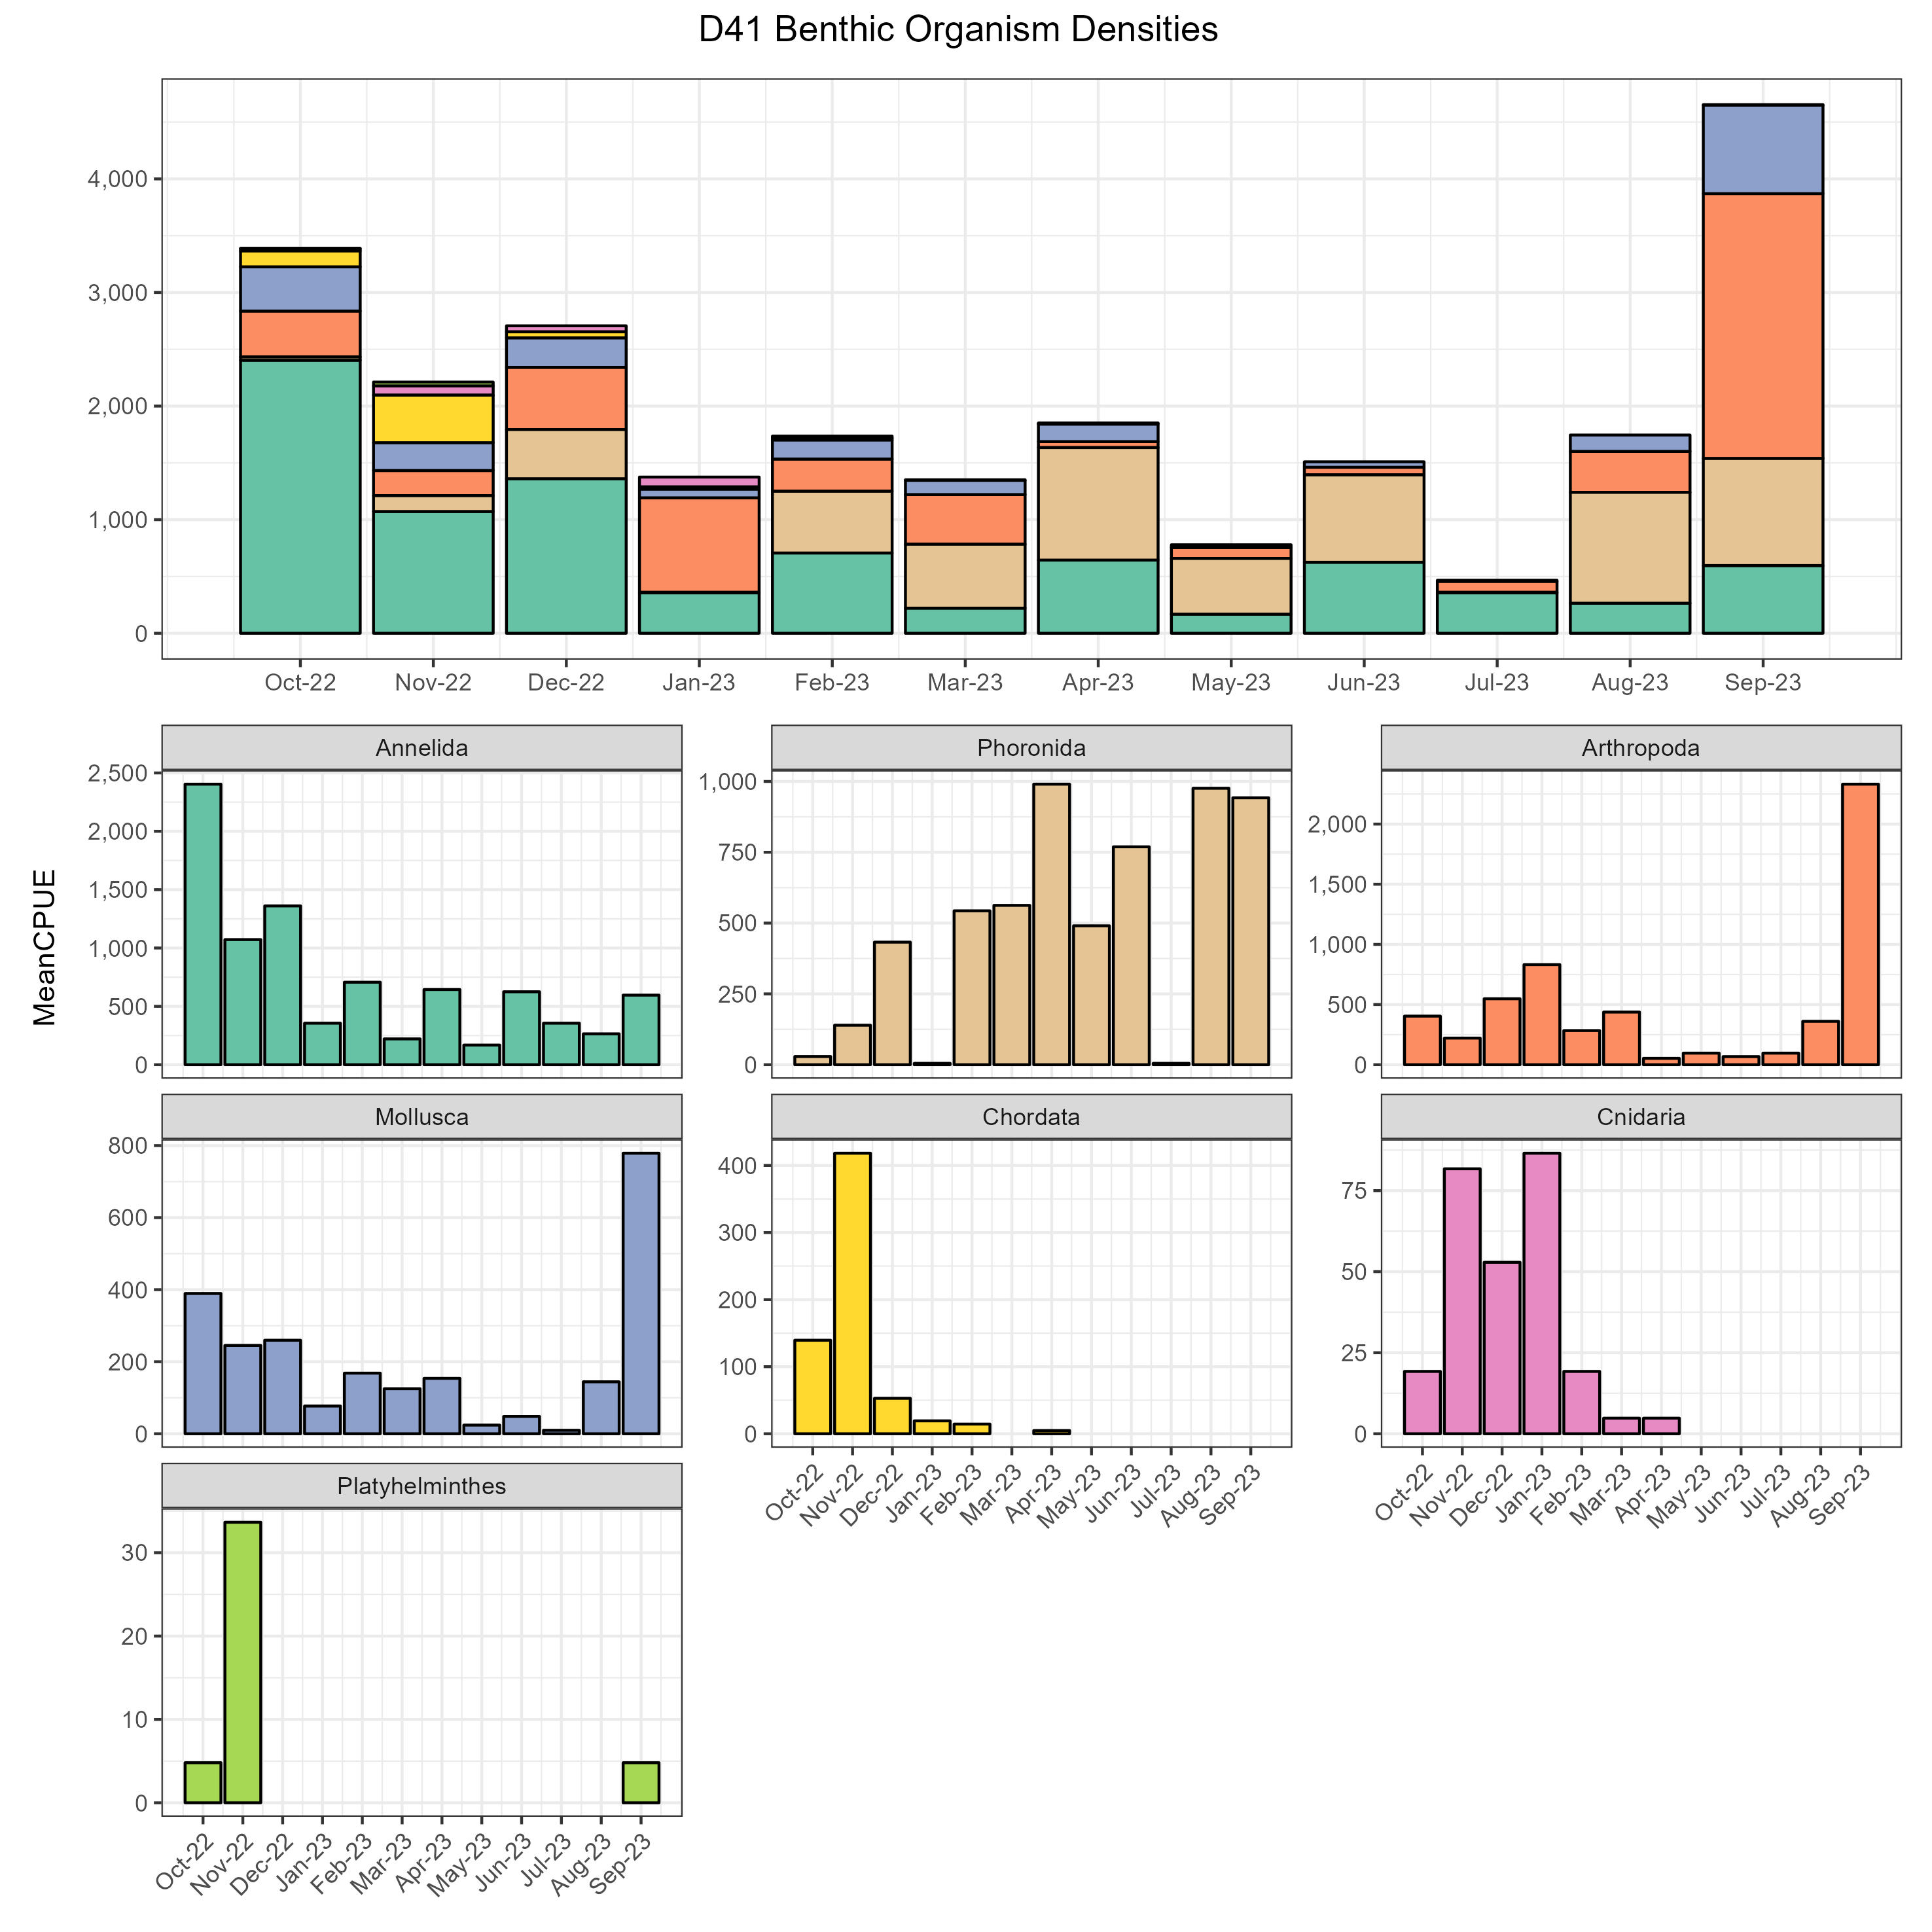
\includegraphics[width=9.84in,height=\textheight]{../figures/benthic_bar_d41.jpg}

}

\caption{\label{fig-benthic_d41}Density of benthic organisms, by month,
collected at station D41.}

\end{figure}

\begin{figure}

{\centering 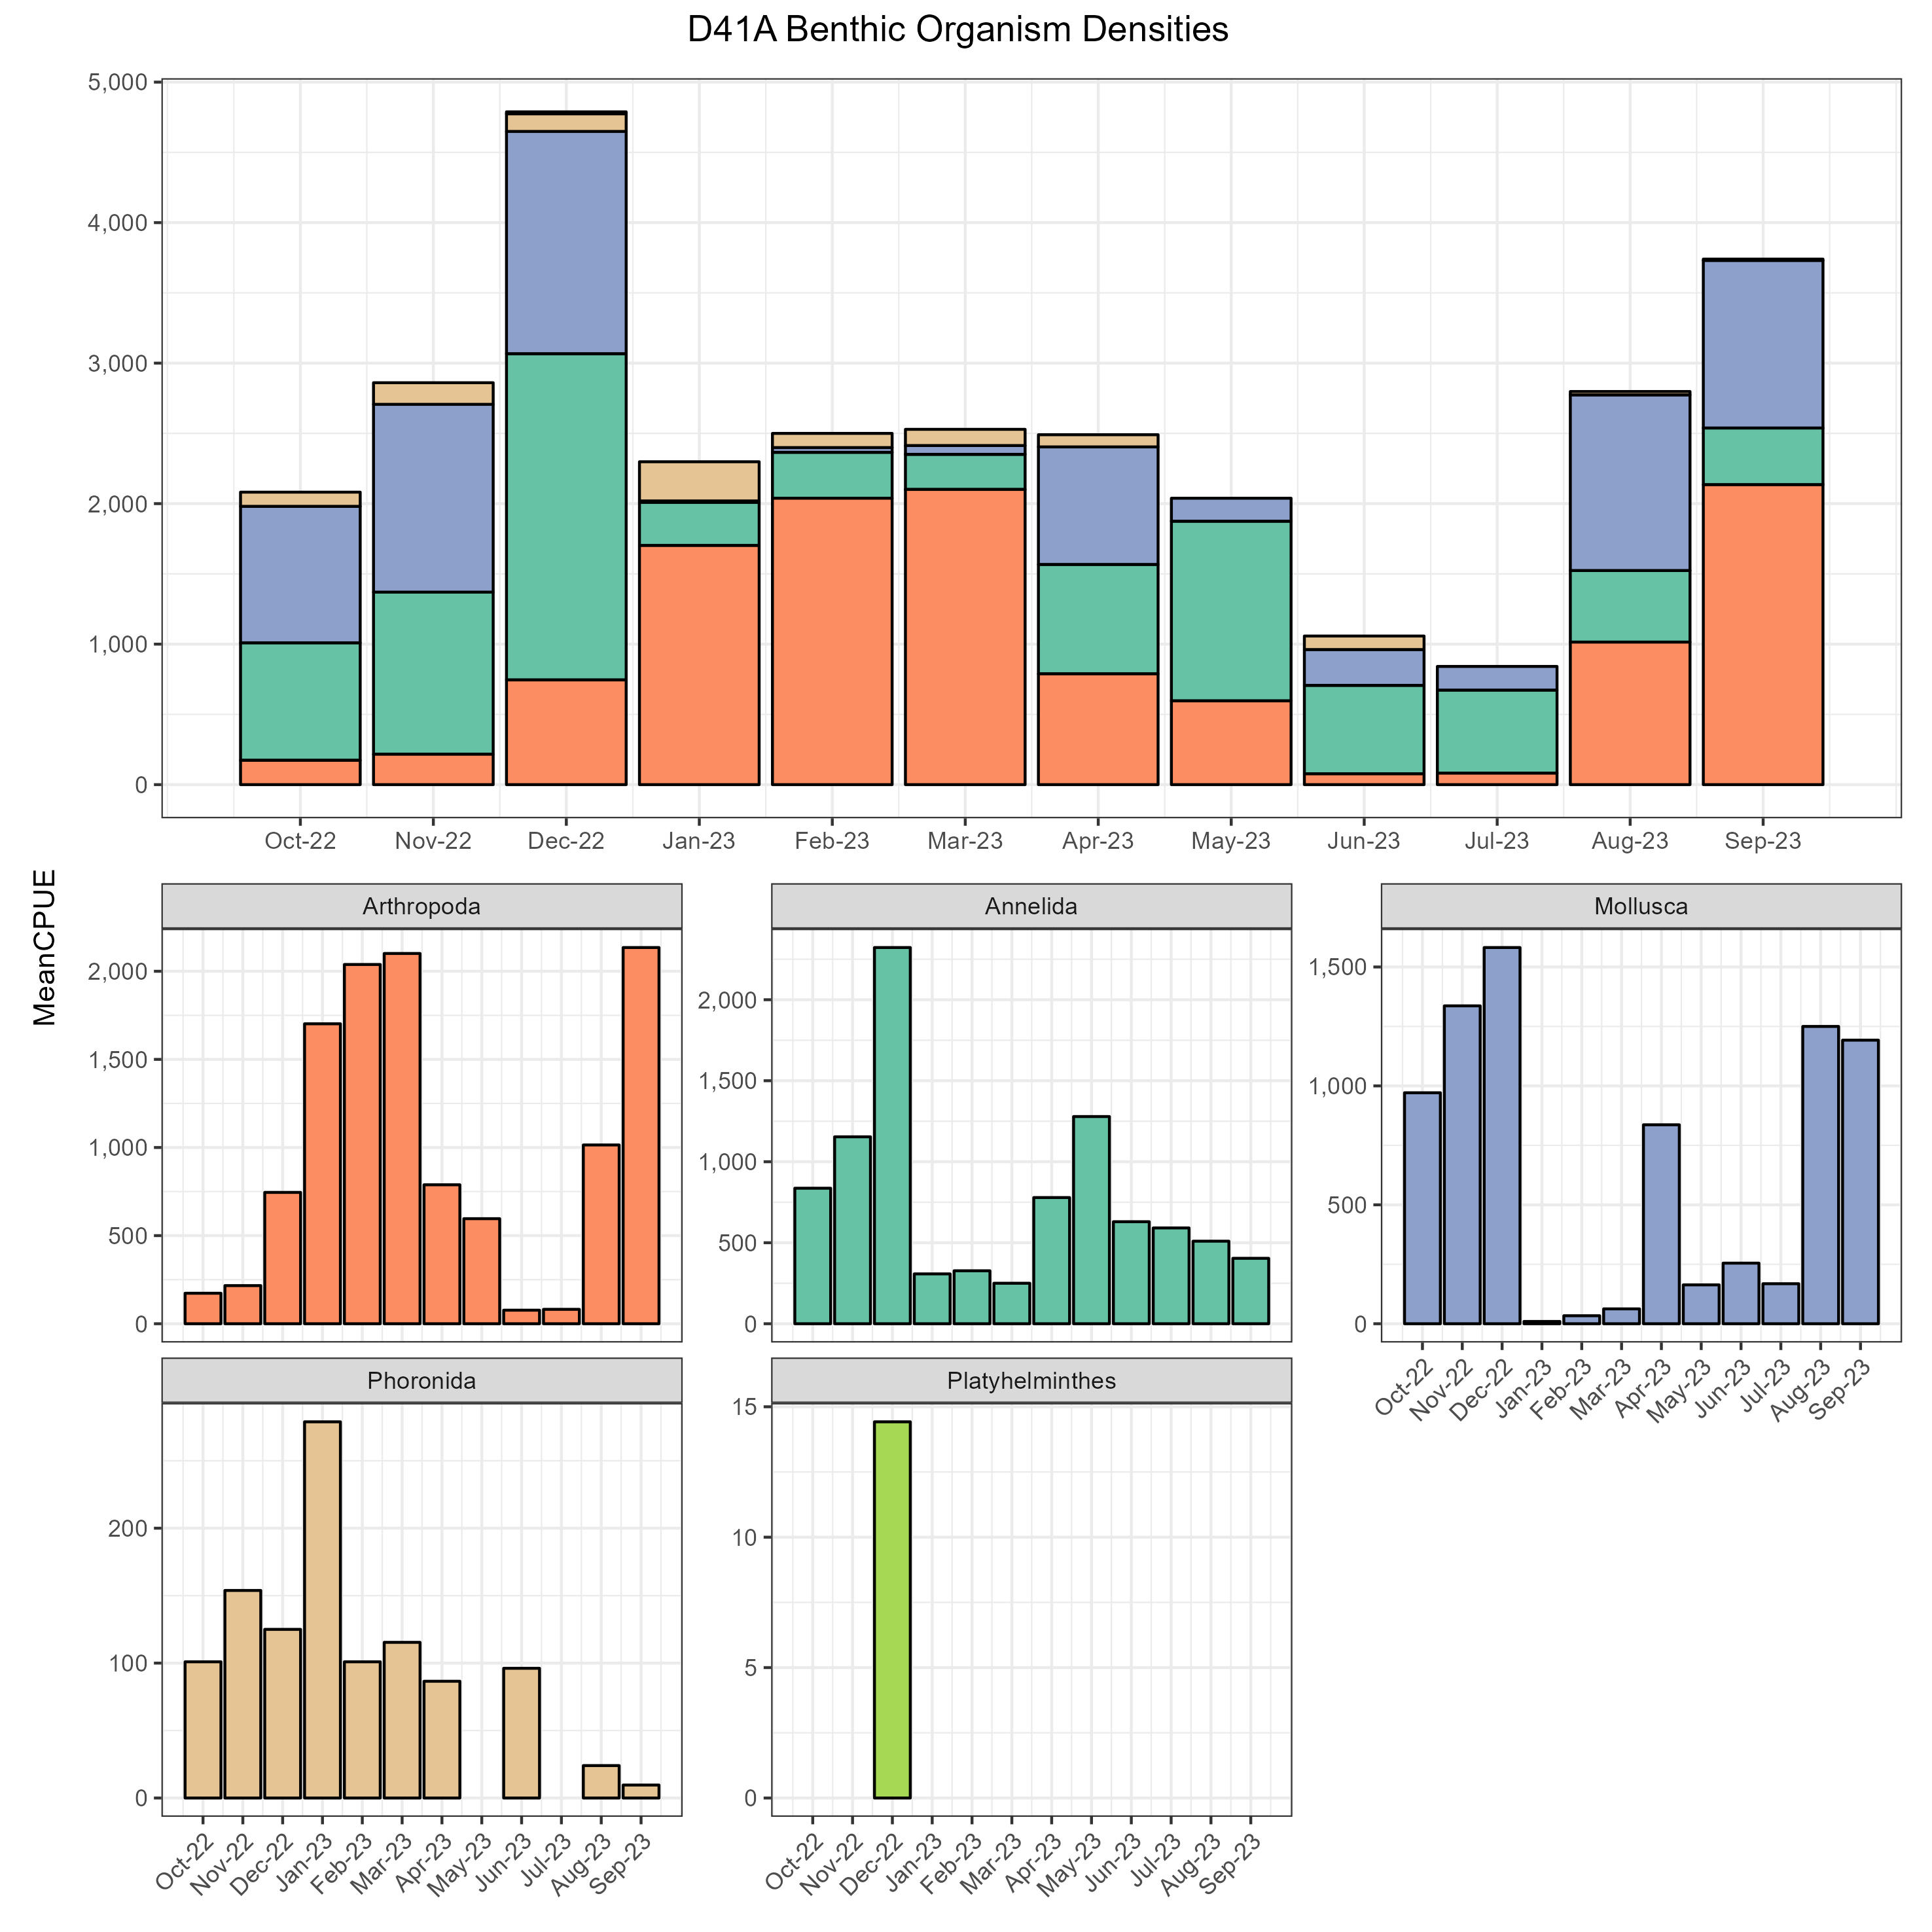
\includegraphics[width=9.84in,height=\textheight]{../figures/benthic_bar_d41a.jpg}

}

\caption{\label{fig-benthic_d41a}Density of benthic organisms, by month,
collected at station D41A.}

\end{figure}

\hypertarget{south-delta-p8-c9}{%
\subsubsection{South Delta (P8, C9)}\label{south-delta-p8-c9}}

The benthic monitoring program sampled at two stations in the South
Delta. Site P8 is on the San Joaquin River at Buckley Cove
(Figure~\ref{fig-stations}). Sampling did not occur in December 2022 due
to very foggy conditions.~ Station P8 had a total of 54 species in five
phyla in WY 2023. Annelida was by far the most abundant phyla at this
station in 2023, accounting for 90\% of all organisms collected
(Figure~\ref{fig-benthic_p8}). The dominant species driving most of the
Annelida patterns was the non-native sabellid worm~\emph{Manayunkia
speciosa}, which had an annual density of 5,501
individuals/m\textsuperscript{2}~and accounted by itself for 59\% of all
organisms.~\emph{Manayunkia speciosa}~in 2023 increased slightly from
its lower densities from 2017 through 2022, but not close to the high
densities seen from 2012 to 2016, which peaked at 11,705
individuals/m\textsuperscript{2}~in WY 2016. The oligochate
worms~\emph{Limnodrilus hoffmeisteri}~and~\emph{Varichaetadrilus
angustipenis}~were the next most common organisms at 1,271 and
537individuals/m\textsuperscript{2}~annual density, followed by a long
tail of many species represented at low densities. This community
composition has remained largely unchanged through the last decade,
apart from the dramatic changes in of~\emph{M. speciosa}.

Site C9 is on Old River at the Clifton Court Forebay intake
(Figure~\ref{fig-stations}). There were 85 species in seven phyla at C9
in WY 2023. Annelida was the dominant phylum throughout the year,
accounting for 79\% of all organisms collected in WY 2023, followed by
15\% Arthropoda. (Figure~\ref{fig-benthic_c9}). An oligochaete
worm,~\emph{Limnodrilus hoffmeisteri,} made up 28\% of all organisms
with an annual density of 1,804 individuals/m\textsuperscript{2}, which
is roughly a quarter of its decade high value in WY 2012 of 5,454
individuals/m\textsuperscript{2}. The oligochaete
worms~\emph{Varichaetadrilus angustipenis} and \emph{Ilyodrilus
frantzi}~were the next most numeous, with average densities of 1,755 and
1,670 individuals/m\textsuperscript{2}. \emph{Limnodrilus}
\emph{hoffmeisteri} and \emph{Ilyodrilus frantzi} had their highest
densities from May through September 2023.~ The freshwater
amphipod~\emph{Hyalella}~sp. A was also notable with an annual average
of 737 individuals/m\textsuperscript{2} through WY 2023, with two peaks
in November 2022 and June 2023. Similar to P8, C9 has a large number of
low-density species, including the highest diversity of aquatic insect
larvae at any site sampled (23 species in WY 2023, mostly chironomid
midges). The community was dominated by oligochaetes and had the same
overall composition as it has for many years.

\begin{figure}

{\centering 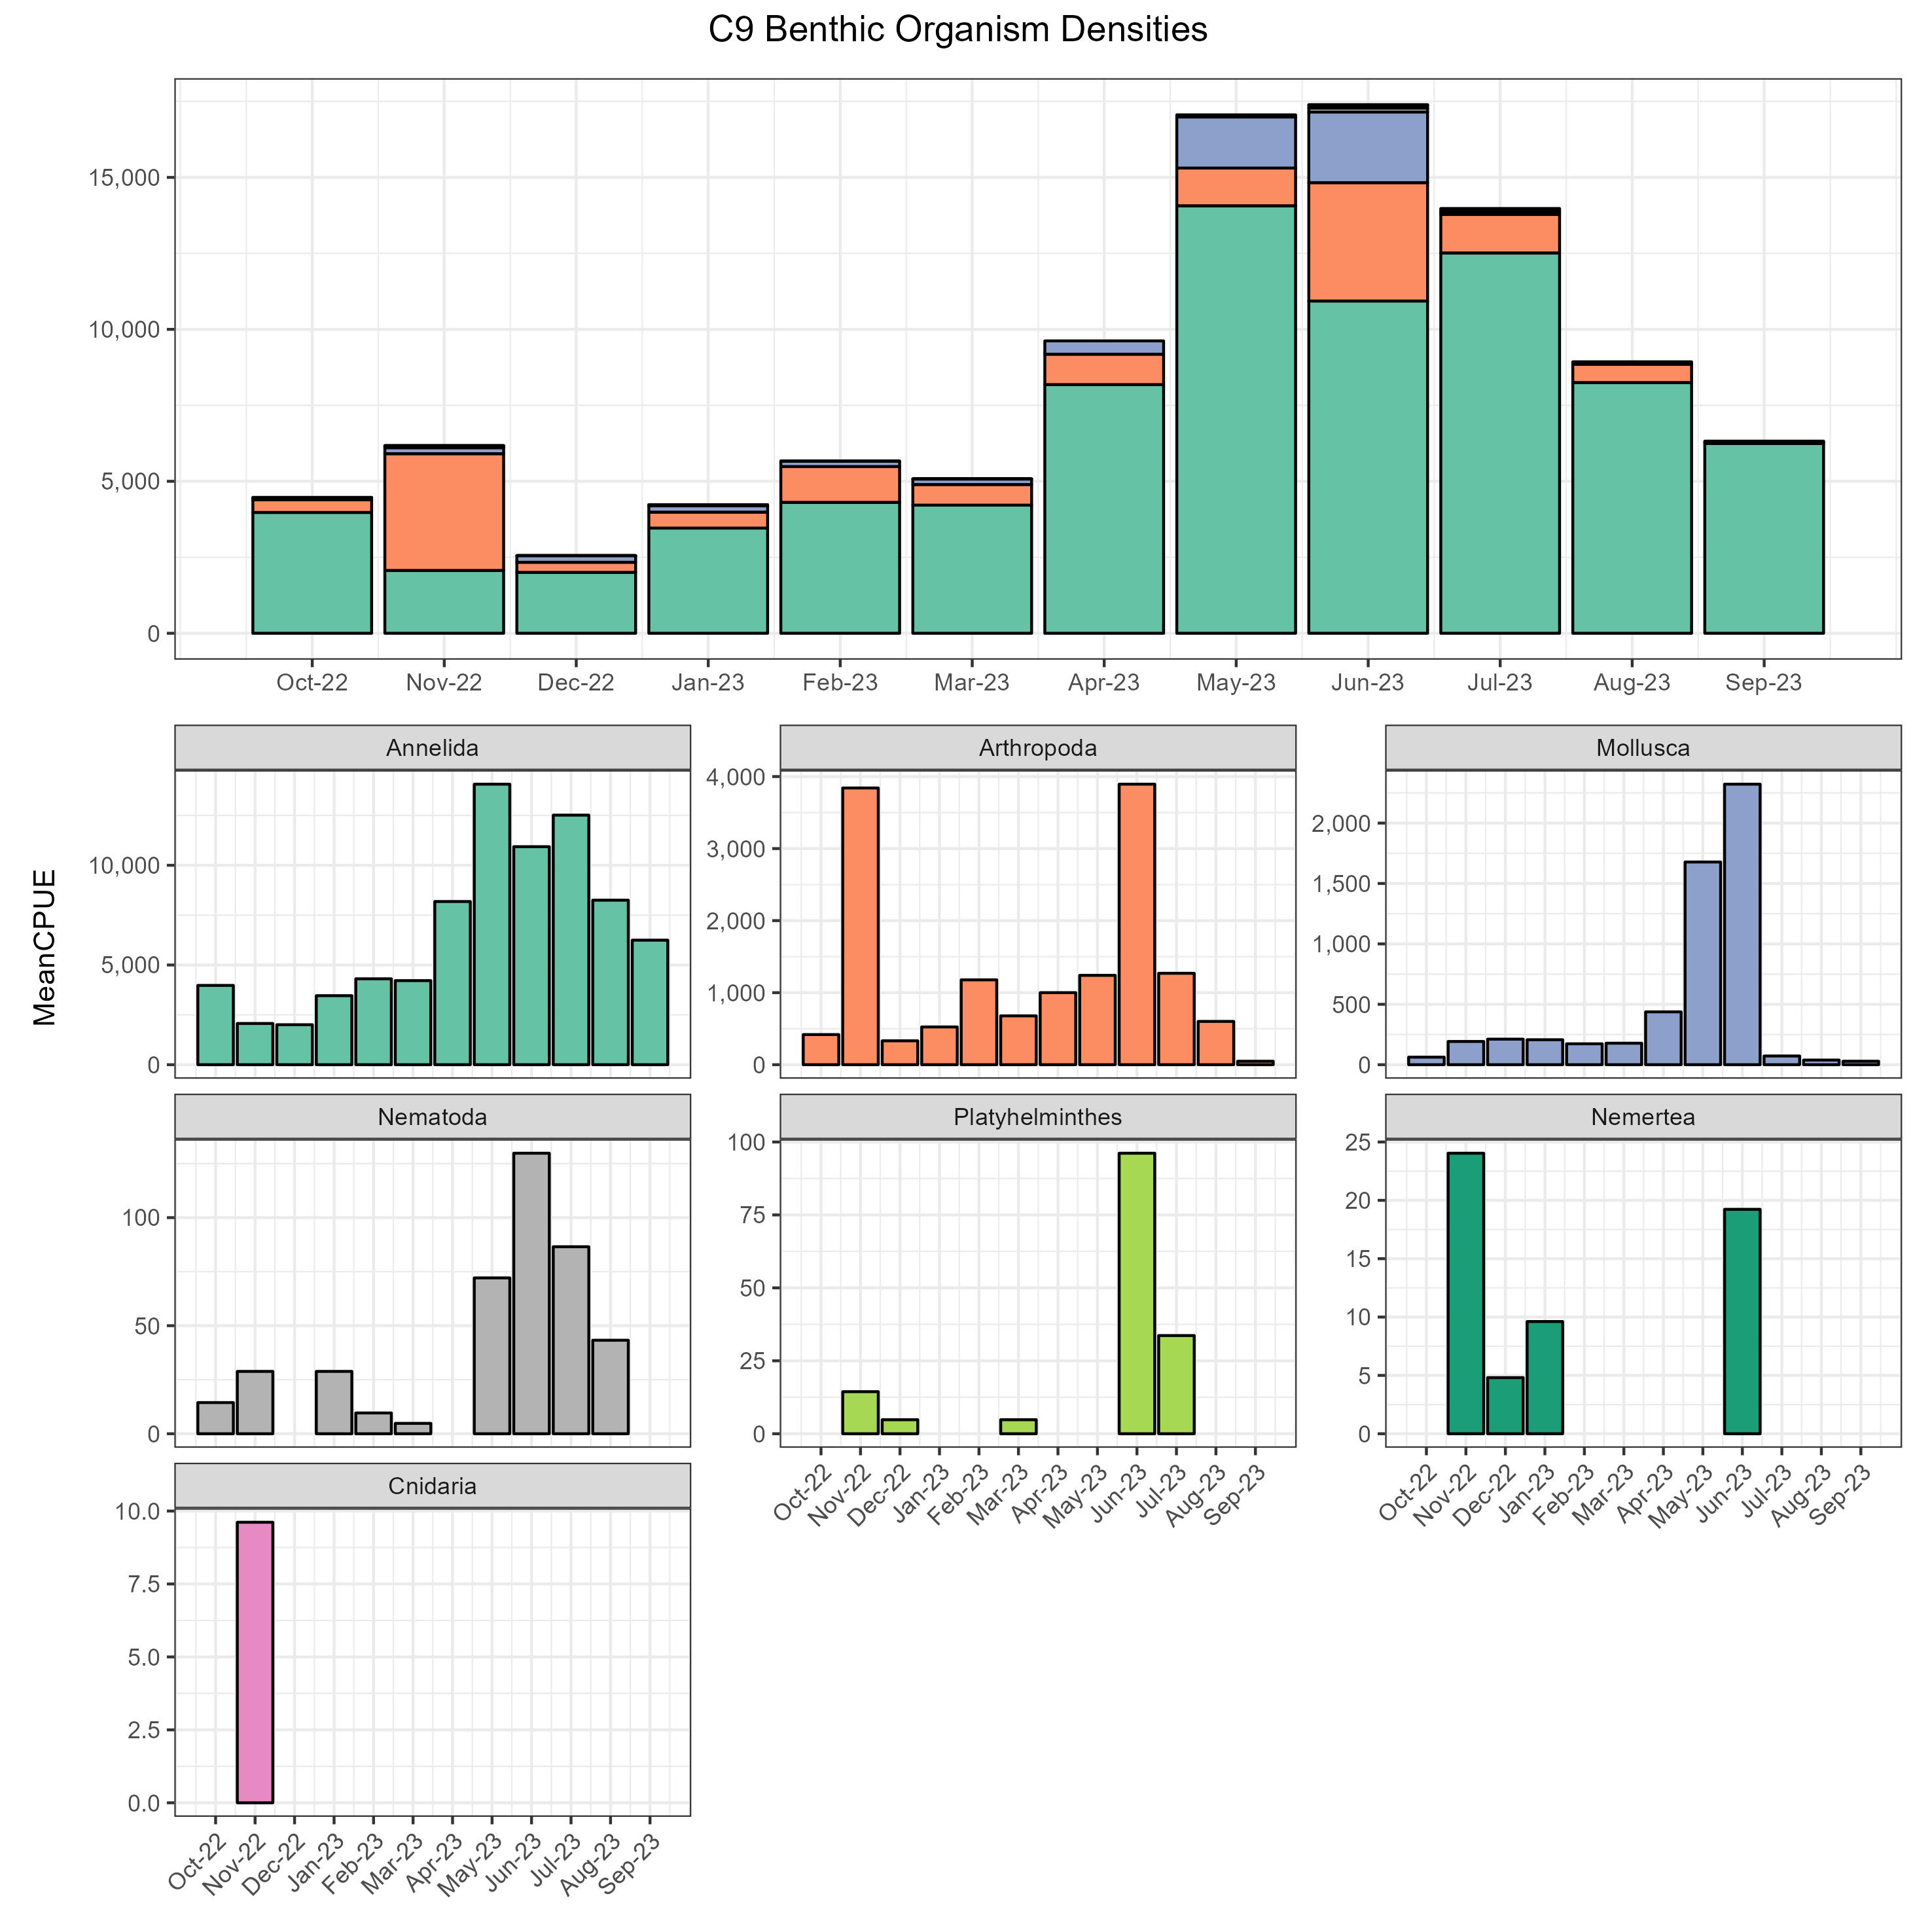
\includegraphics[width=9.84in,height=\textheight]{../figures/benthic_bar_c9.jpg}

}

\caption{\label{fig-benthic_c9}Density of benthic organisms, by month,
collected at station C9.}

\end{figure}

\begin{figure}

{\centering 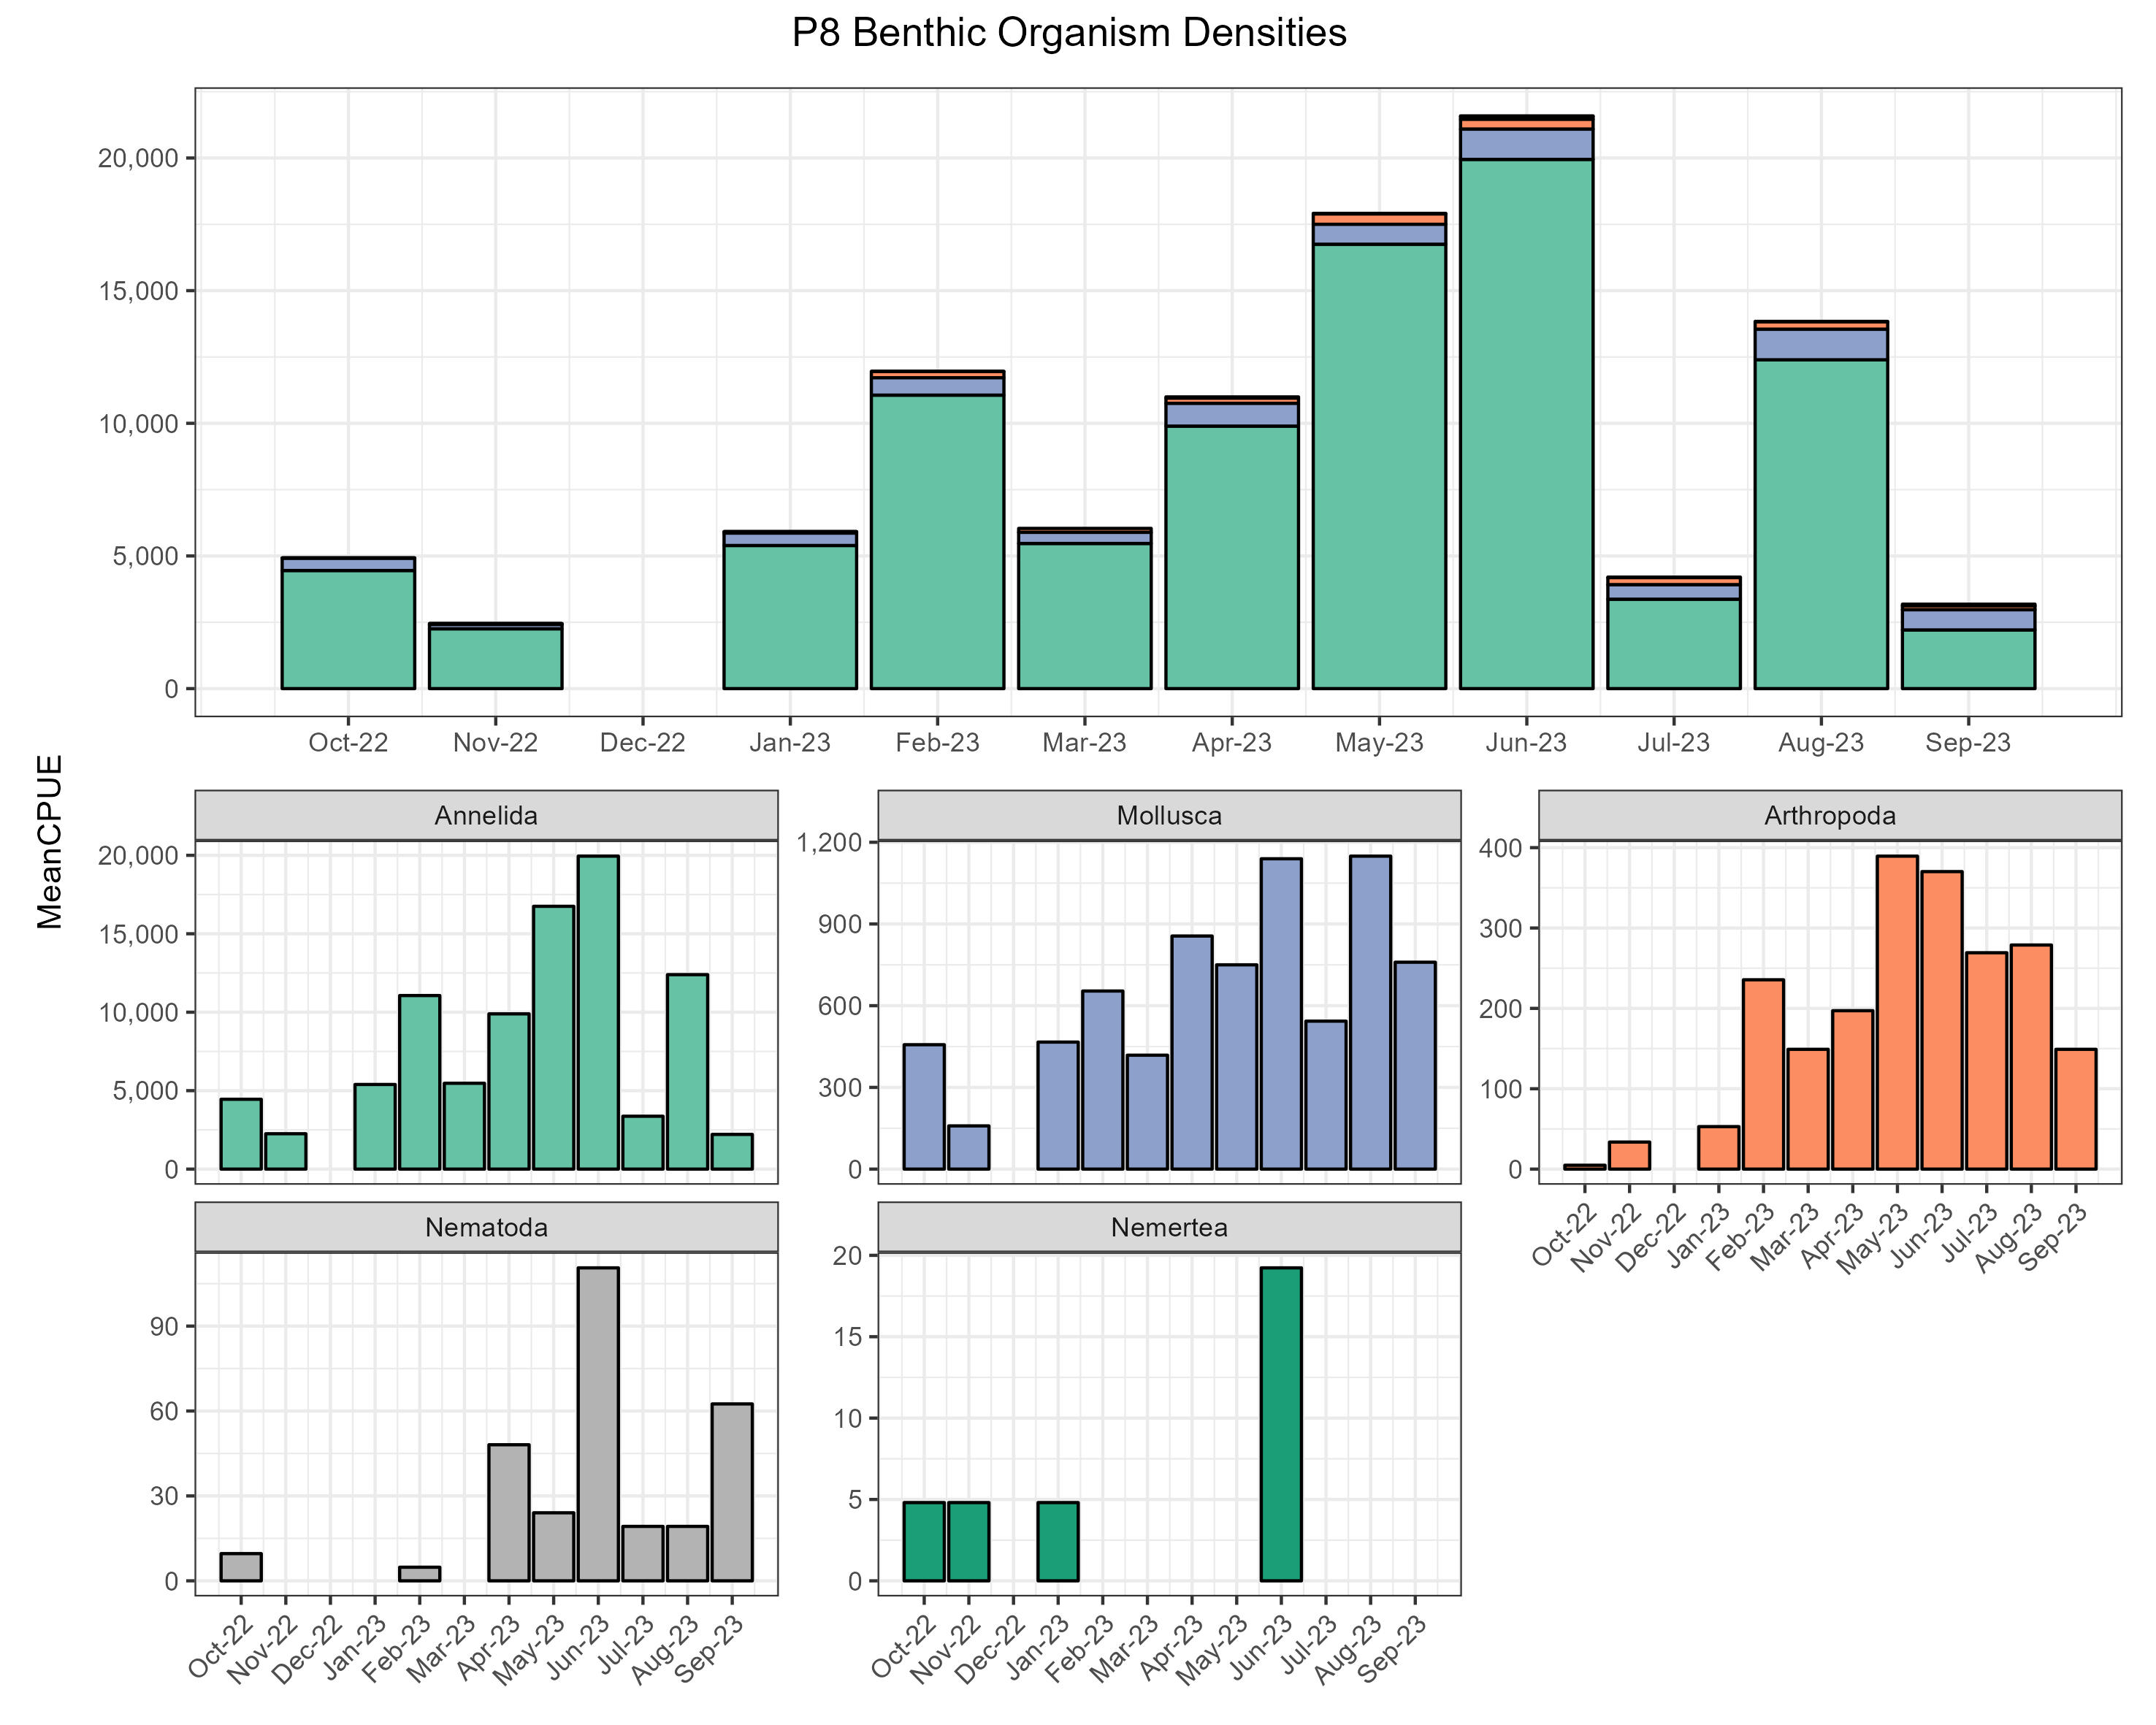
\includegraphics[width=9.84in,height=\textheight]{../figures/benthic_bar_p8.jpg}

}

\caption{\label{fig-benthic_p8}Density of benthic organisms, by month,
collected at station P8.}

\end{figure}

\hypertarget{suisun-grizzly-bays-d6-d7}{%
\subsubsection{Suisun \& Grizzly Bays (D6,
D7)}\label{suisun-grizzly-bays-d6-d7}}

The benthic monitoring program sampled at two stations in the Suisun Bay
area, D6 and D7. Site D6 is in Suisun Bay near the I-680 bridge
(Figure~\ref{fig-stations}) and had 28 species in five phyla in WY 2023.
Mollusca was the dominant phylum, accounting for 97\% of all organisms
collected (Figure~\ref{fig-benthic_d6}). Most of the organisms collected
were the invasive Asian clam~\emph{Potamocorbula amurensis}, which had
an annual density of 9,345 individuals/m\textsuperscript{2}, in an
increase from its decade-long low in WY 2017 but still below its WY 2020
high of 23,800 individuals/m\textsuperscript{2}.~\emph{Potamocorbula
amurensis}~was most abundant in August 2023 with 55,548
individuals/m\textsuperscript{2}, likely as a result of summer seasonal
recruitment. The relatively few other organisms found at this site were
predominately from phylum Arthropoda, either the brackish-water bay
barnacle~\emph{Amphibalanus improvisus}, found mostly growing
on~\emph{P. amurensis}~shells, or the cumacean crustacean
\emph{Nippoleucon hinumensis}.

Site D7 is in Grizzly Bay, near the entrance to Suisun Slough
(Figure~\ref{fig-stations}). There were 29 species in three phyla in WY
2023. Mollusca comprised 64\% of the total organisms, Arthropoda 28\%,
and Annelida 8\%. The non-native clam~\emph{Potamocorbula amurensis} and
the cumacean arthropod~\emph{Nippoleucon hinumensis}~were the two most
abundant species, comprising 64\% and 21\% of the total community
through the year, respectively
(Figure~\ref{fig-benthic_d7}).~\emph{Nippoleucon hinumensis}~had an
annual density of 673 organisms/m\textsuperscript{2}, but saw a strong
seasonal pattern: relatively high densities from October through
December and relatively lower densities the rest of the year, including
almost none from June through September.~\emph{Potamocorbula
amurensis}~had an annual average density of
2,085/organisms/m\textsuperscript{2} and a very strongly seasonal
pattern as well -- high numbers in October 20022 decreasing through
winter and spring, then an abrupt increase in seasonal recruitment in
August to 9,284 organisms/m\textsuperscript{2}. While~\emph{P.
amurensis}~has been numerically dominant through the last decade, a
major change in WY 2021 was the rise of~\emph{N. hinumensis}~and a
simultaneous crash of the amphipod~\emph{Sinocorophium alienense}, which
had been the second-densest species at D7 for at least the last
decade.~\emph{Sinocorophium alienense}~crashed in WY 2021 to around 576
organisms/m\textsuperscript{2}, was completely absent from D7 in WY
2022, and barely appeared in WY 2023 at all.

\begin{figure}

{\centering 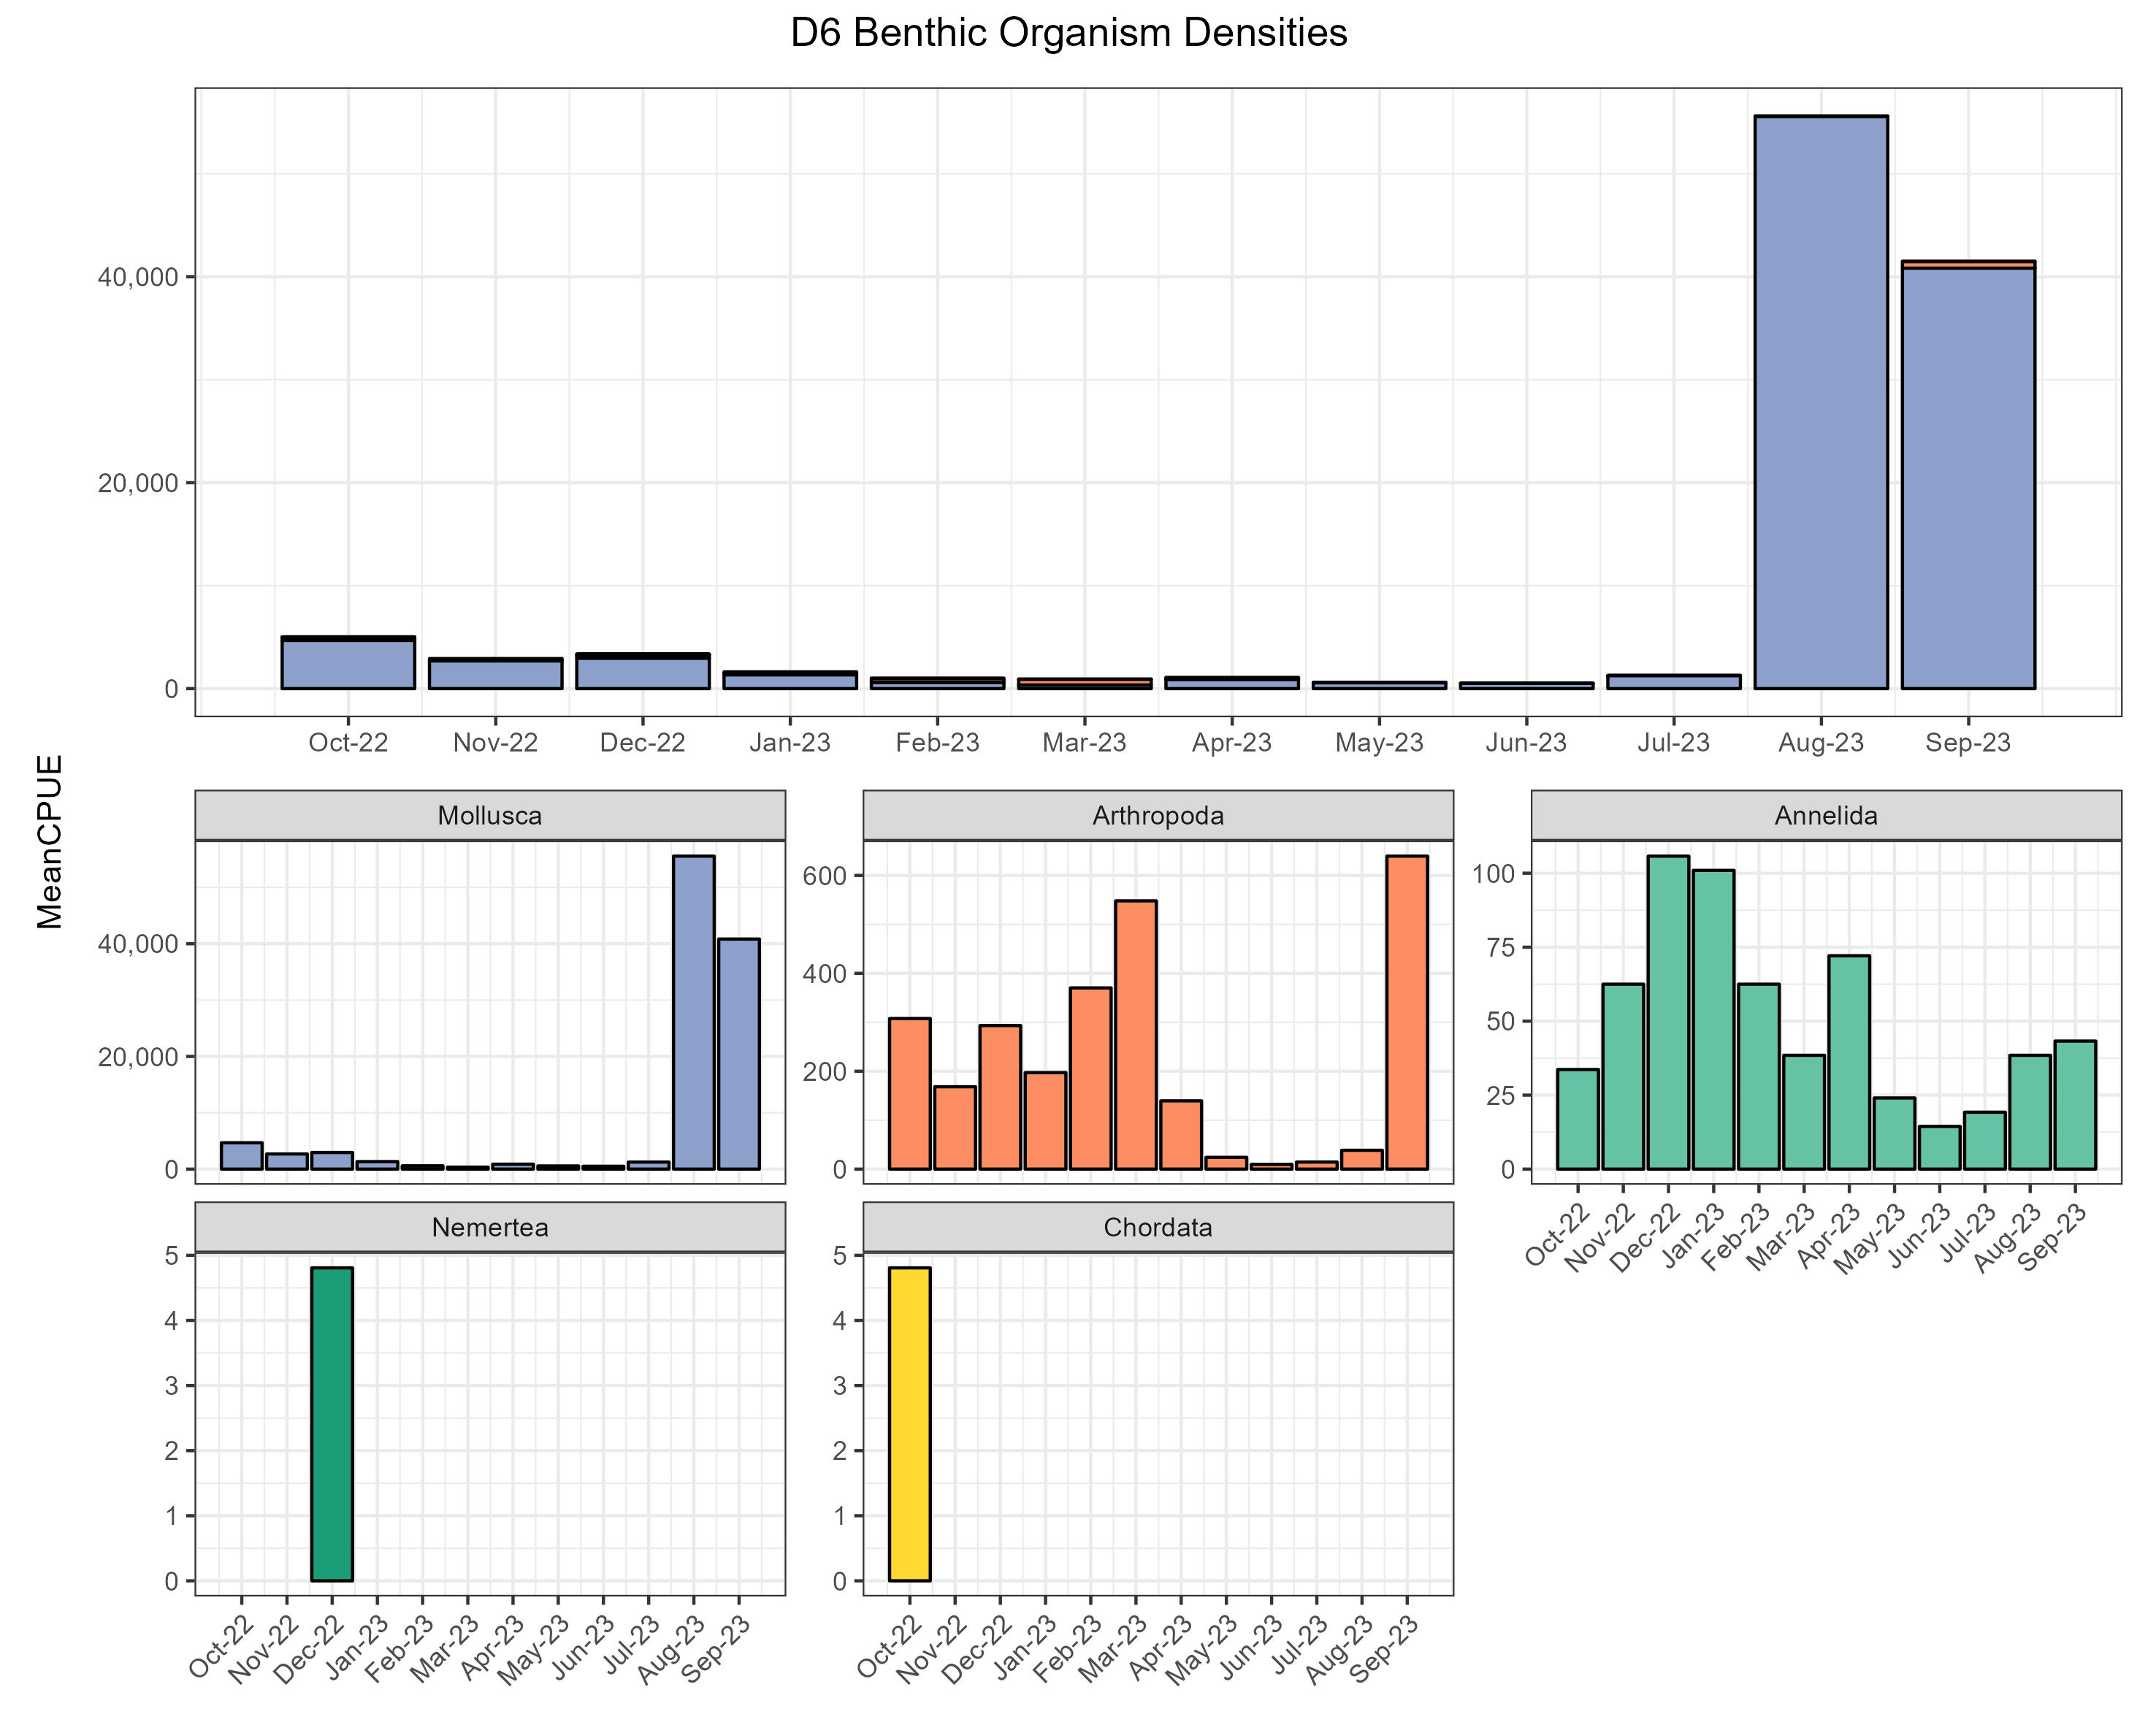
\includegraphics[width=9.84in,height=\textheight]{../figures/benthic_bar_d6.jpg}

}

\caption{\label{fig-benthic_d6}Density of benthic organisms, by month,
collected at station D6.}

\end{figure}

\begin{figure}

{\centering 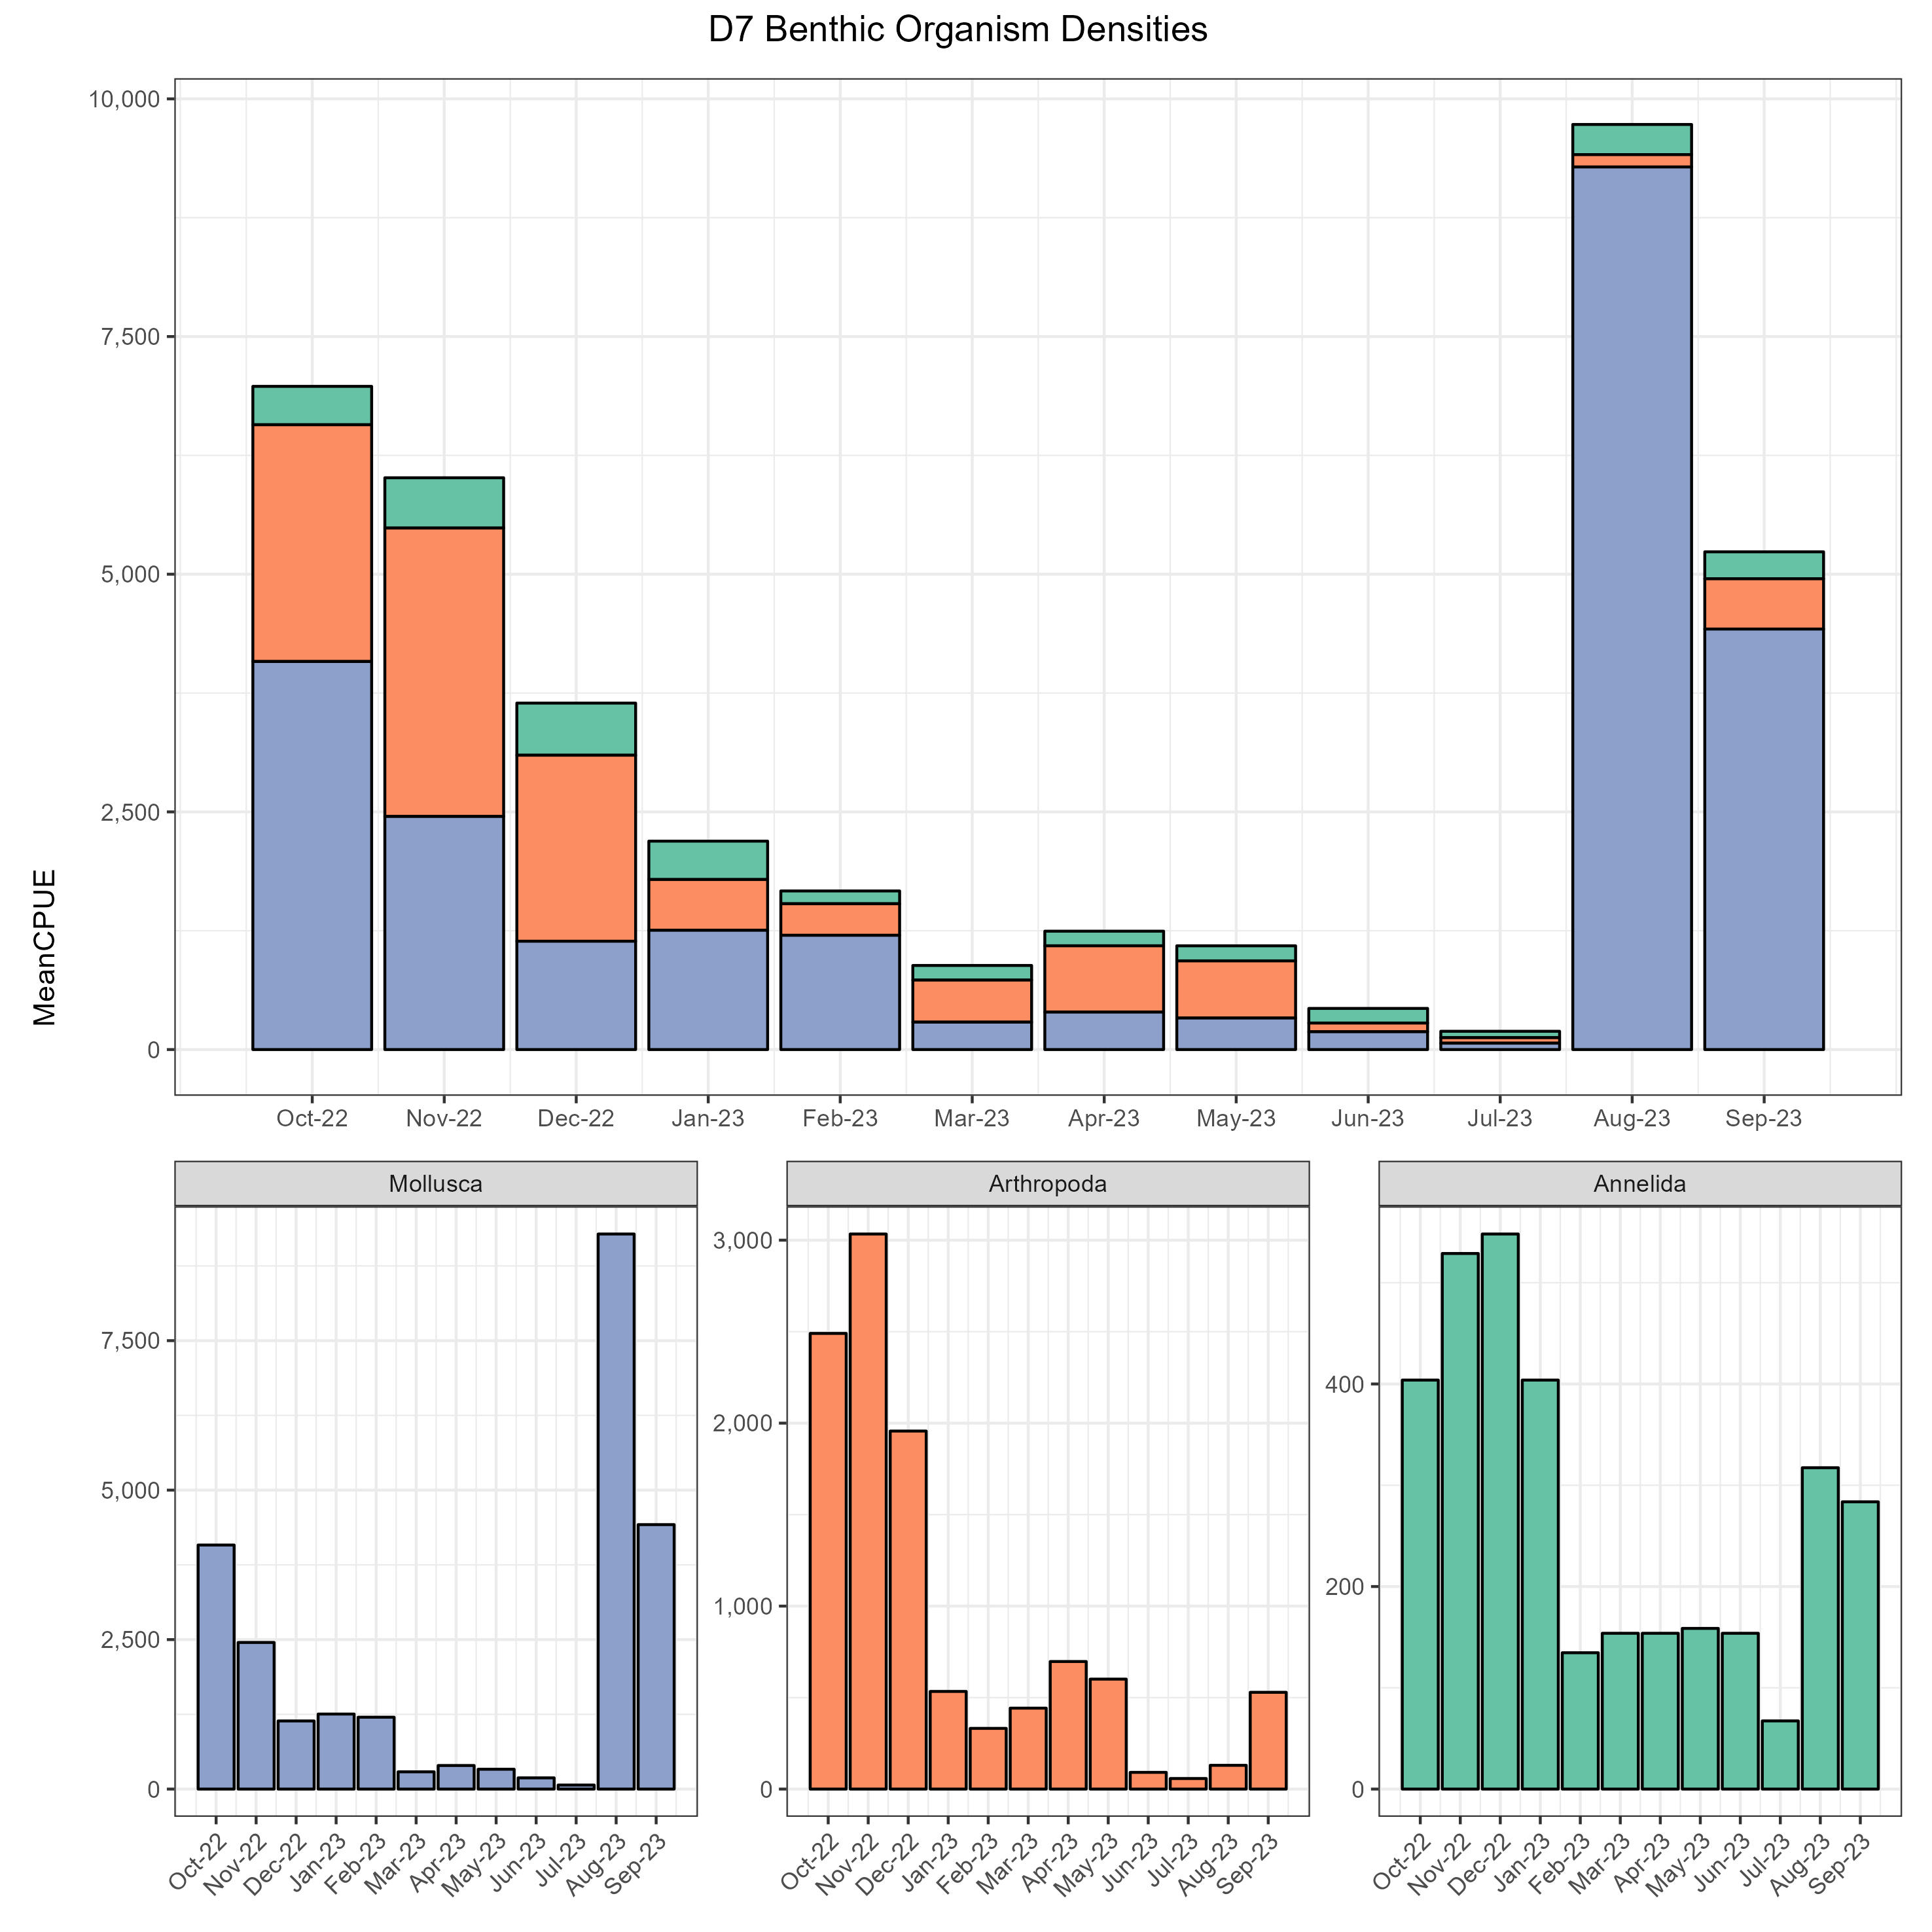
\includegraphics[width=9.84in,height=\textheight]{../figures/benthic_bar_d7.jpg}

}

\caption{\label{fig-benthic_d7}Density of benthic organisms, by month,
collected at station D7.}

\end{figure}

\hypertarget{interpretations}{%
\subsection{Interpretations}\label{interpretations}}

In summary, WY 2023 saw the second lowest average organism density of
any year of the past decade, second only to WY 2022. This trend was
consistent across most sites, and was caused largely by the decrease in
various amphipod species, especially~\emph{Ampelisca abdita}~in San
Pablo Bay and~\emph{Sinocorophium alienense}~in Grizzly Bay, as well as
the decrease in the sabellid worm \emph{Manayunkia speciosa} at Central
Delta sites. Since many fish species have switched to amphipod food
sources after the collapse of mysid shrimps (Feyrer et al.~2003), the
near disappearance of various amphipod species may have food web
implications unless they have simply shifted their ranges out of our
sampling area. Densities of the non-native clams \emph{Potamocorbula
amurensis} and \emph{Corbicula fluminea} were also near decade lows in
WY 2023, possibly because of the wet water year 2023, which caused clams
to shift ranges downstream and their numbers to be depressed until they
could recruit in the following warm season to their new salinity
ranges.~ Ordinarily, the decrease of both species of invasive clams and
their filter-feeding activity would be a favorable sign for the
ecosystem, but the relative absence of several other numerically
dominant members of the community in WY 2023 has unclear implications.
Our ability to recognize these changes over decadal timescales
highlights the importance of continued monitoring of benthic
invertebrates to a high taxonomic resolution across the entire estuarine
salinity gradient, as the community interacts with both various abiotic
conditions as well as key parts of the estuarine food web.

\hypertarget{references}{%
\subsection{References}\label{references}}

Fields W, Messer C. 1999. Life on the bottom: Trends in species
composition of the IEP-DWR Benthic Monitoring Program. IEP Newsletter
12(4): 38-41.

Carlton, J. T. 2007. The Light and Smith manual: Intertidal
Invertebrates from central California to Oregon, 4th edition. Berkeley,
CA, University of California Press.

Feyrer, F., B. Herbold, S. A. Matern and P. B. Moyle. 2003. Dietary
shifts in a stressed fish assemblage: consequences of a bivalve invasion
in the San Francisco Estuary. Environmental Biology of Fishes 67(3):
277-288.

\hypertarget{archived-reports}{%
\subsection{Archived Reports}\label{archived-reports}}

Previous EMP benthic reports can be found
\href{https://github.com/emp-dwr/emp-website/tree/gh-pages/admin/archive/benthic}{here}.



\end{document}
